% Options for packages loaded elsewhere
\PassOptionsToPackage{unicode}{hyperref}
\PassOptionsToPackage{hyphens}{url}
\PassOptionsToPackage{dvipsnames,svgnames,x11names}{xcolor}
\documentclass[
  10pt,
]{article}
\usepackage{xcolor}
\usepackage[margin=2.2cm]{geometry}
\usepackage{amsmath,amssymb}
\setcounter{secnumdepth}{-\maxdimen} % remove section numbering
\usepackage{iftex}
\ifPDFTeX
  \usepackage[T1]{fontenc}
  \usepackage[utf8]{inputenc}
  \usepackage{textcomp} % provide euro and other symbols
\else % if luatex or xetex
  \usepackage{unicode-math} % this also loads fontspec
  \defaultfontfeatures{Scale=MatchLowercase}
  \defaultfontfeatures[\rmfamily]{Ligatures=TeX,Scale=1}
\fi
\usepackage{lmodern}
\ifPDFTeX\else
  % xetex/luatex font selection
\fi
% Use upquote if available, for straight quotes in verbatim environments
\IfFileExists{upquote.sty}{\usepackage{upquote}}{}
\IfFileExists{microtype.sty}{% use microtype if available
  \usepackage[]{microtype}
  \UseMicrotypeSet[protrusion]{basicmath} % disable protrusion for tt fonts
}{}
\makeatletter
\@ifundefined{KOMAClassName}{% if non-KOMA class
  \IfFileExists{parskip.sty}{%
    \usepackage{parskip}
  }{% else
    \setlength{\parindent}{0pt}
    \setlength{\parskip}{6pt plus 2pt minus 1pt}}
}{% if KOMA class
  \KOMAoptions{parskip=half}}
\makeatother
\usepackage{listings}
\newcommand{\passthrough}[1]{#1}
\lstset{defaultdialect=[5.3]Lua}
\lstset{defaultdialect=[x86masm]Assembler}
\usepackage{longtable,booktabs,array}
\usepackage{calc} % for calculating minipage widths
% Correct order of tables after \paragraph or \subparagraph
\usepackage{etoolbox}
\makeatletter
\patchcmd\longtable{\par}{\if@noskipsec\mbox{}\fi\par}{}{}
\makeatother
% Allow footnotes in longtable head/foot
\IfFileExists{footnotehyper.sty}{\usepackage{footnotehyper}}{\usepackage{footnote}}
\makesavenoteenv{longtable}
\usepackage{graphicx}
\makeatletter
\newsavebox\pandoc@box
\newcommand*\pandocbounded[1]{% scales image to fit in text height/width
  \sbox\pandoc@box{#1}%
  \Gscale@div\@tempa{\textheight}{\dimexpr\ht\pandoc@box+\dp\pandoc@box\relax}%
  \Gscale@div\@tempb{\linewidth}{\wd\pandoc@box}%
  \ifdim\@tempb\p@<\@tempa\p@\let\@tempa\@tempb\fi% select the smaller of both
  \ifdim\@tempa\p@<\p@\scalebox{\@tempa}{\usebox\pandoc@box}%
  \else\usebox{\pandoc@box}%
  \fi%
}
% Set default figure placement to htbp
\def\fps@figure{htbp}
\makeatother
\setlength{\emergencystretch}{3em} % prevent overfull lines
\providecommand{\tightlist}{%
  \setlength{\itemsep}{0pt}\setlength{\parskip}{0pt}}
\usepackage{etoolbox}
\AtBeginEnvironment{longtable}{\footnotesize}
\lstset{basicstyle=\ttfamily\footnotesize,breaklines=true,columns=fullflexible,frame=single}
\setlength{\emergencystretch}{3em}
\renewcommand{\topfraction}{0.9}
\renewcommand{\textfraction}{0.07}
\renewcommand{\floatpagefraction}{0.8}
\usepackage{bookmark}
\IfFileExists{xurl.sty}{\usepackage{xurl}}{} % add URL line breaks if available
\urlstyle{same}
\hypersetup{
  pdftitle={OMC at TREC 2026 AutoJudge: Probabilistic Pairwise, Graded-Rubric and Grounding-Discounted Judges with Jev},
  pdfauthor={Team omc26},
  colorlinks=true,
  linkcolor={Maroon},
  filecolor={Maroon},
  citecolor={Blue},
  urlcolor={Blue},
  pdfcreator={LaTeX via pandoc}}

\title{OMC at TREC 2026 AutoJudge: Probabilistic Pairwise, Graded-Rubric
and Grounding-Discounted Judges with Jev}
\usepackage{etoolbox}
\makeatletter
\providecommand{\subtitle}[1]{% add subtitle to \maketitle
  \apptocmd{\@title}{\par {\large #1 \par}}{}{}
}
\makeatother
\subtitle{Methods and results (notebook paper draft)}
\author{Team omc26}
\date{Draft, 30 October 2026}

\begin{document}
\maketitle

\subsection{1. Overview}\label{overview}

\textbf{Authors:} Max Irwin
\href{mailto:max@onemorecloud.com}{\nolinkurl{max@onemorecloud.com}},
Nathan Day \href{mailto:nday@eezy.com}{\nolinkurl{nday@eezy.com}},
Daniel Worley
\href{mailto:dworley@gmail.com}{\nolinkurl{dworley@gmail.com}}

\textbf{Introduction:} For TREC AutoJudge 2026, covering the rag26 and
ragtime26 tracks, we took approaches to directly construct leaderboards
for the tracks by grading of RAG summary output. For this meta-judge
approach, we had two primary constraints to work with: (a) no existing
golden set for the leaderboard task and (b) a limited window of
responses to prevent LLM data leakage and overfitting. We submitted 10
hypotheses' outputs. We performed this task ``in the dark'' awaiting
final results from the official TREC judges, and this forced us down
several interesting paths using (1) new tools such as System One models
(aka ``Jev''), (2) SOTA practitioner techniques such as pairwise and
bag-of-decisions auto-grading, and (3) classical tools such as SpaCy for
concept hallucination risk. Along the way, we pulled apart Jev and
discovered biases, found key restrictions of costs and speed with
private LLMs, and saw interesting result correlations across independent
experiments.

We submitted three judges to both TREC 2026 AutoJudge datasets (rag26
and ragtime26). None was trained or tuned on the evaluation topics
outside a fixed 10-topic window. All three use TypeSafe's \textbf{Jev}
decision model (\passthrough{\lstinline!typesafe/jev-1.13!}), which
returns probabilities instead of generated text.

Our Judges and methods include pairwise preference with several
variants, bag-of-decisions (``BOD'') grading, and lexical concept
overlap (``Hallucination Risk''). At first, we started with lexical
experiments and then used Gemini. The System One model Jev was released
during the competition, and given the high cost and high latency of
Gemini, we pivoted to Jev. We were able to use the Gemini result data as
an agreement point for some of our methods.

\begin{longtable}[]{@{}
  >{\raggedright\arraybackslash}p{(\linewidth - 8\tabcolsep) * \real{0.4453}}
  >{\raggedright\arraybackslash}p{(\linewidth - 8\tabcolsep) * \real{0.1396}}
  >{\raggedright\arraybackslash}p{(\linewidth - 8\tabcolsep) * \real{0.2189}}
  >{\raggedright\arraybackslash}p{(\linewidth - 8\tabcolsep) * \real{0.1094}}
  >{\raggedright\arraybackslash}p{(\linewidth - 8\tabcolsep) * \real{0.0868}}@{}}
\toprule\noalign{}
\begin{minipage}[b]{\linewidth}\raggedright
Judge
\end{minipage} & \begin{minipage}[b]{\linewidth}\raggedright
Unit judged
\end{minipage} & \begin{minipage}[b]{\linewidth}\raggedright
Primary measure
\end{minipage} & \begin{minipage}[b]{\linewidth}\raggedright
Jev calls (rag26 / ragtime26)
\end{minipage} & \begin{minipage}[b]{\linewidth}\raggedright
API cost, both datasets
\end{minipage} \\
\midrule\noalign{}
\endhead
\bottomrule\noalign{}
\endlastfoot
\textbf{Pairwise:} mirrored, depth-proportionate yes/no questions, both
orientations & pair of reports, cross-team &
\passthrough{\lstinline!PAIRWISE\_WINRATE!}: mean over topics of
per-topic win rate & 703,536 / 196,958 unique & \$93.84 \\
\textbf{BOD:} bag-of-decisions graded rubric & one report against a
per-topic rubric & \passthrough{\lstinline!BOD\_MEAN!}: mean expected
grade / 3 & 9,838 / 5,041 answers & \$1.31 \\
\textbf{BOD \ensuremath{\times} Hallucination Risk} & one report &
\passthrough{\lstinline!BOD\_GROUNDED!} =
\passthrough{\lstinline!BOD\_MEAN!} \ensuremath{\times} (1 -
\passthrough{\lstinline!HALLUC\_RISK!}) & 0 new (reuses the BOD grades)
& \$0 \\
\end{longtable}

\textbf{Main results} (details in §§4--8):

\begin{enumerate}
\def\labelenumi{\arabic{enumi}.}
\setcounter{enumi}{1}
\tightlist
\item
  \textbf{Jev has a strong position bias on the first slot for choice},
  and a mirrored pair of yes/no questions fixes the bias.
\item
  \textbf{None of our judges rewards uninformative length} in a
  controlled padding test. Each credits added relevant content, except
  our Gemini baseline on ragtime26.
\item
  \textbf{A ``depth-proportionate'' wording makes the pairwise judge
  respond to how narrow a request is,} on 10 of 10 window topics of each
  dataset.
\item
  \textbf{The rubric judge (BOD) agrees with the pairwise judge} at
  \ensuremath{\rho} 0.991 (rag26) and 0.943 (ragtime26) over all topics,
  at about 1/70 of the cost.
\item
  \textbf{The hallucination discount is small} (median risk about 1\%)
  but changes the top-ranked run on both datasets.
\end{enumerate}

\begin{center}\rule{0.5\linewidth}{0.5pt}\end{center}

\subsection{2. Task and data}\label{task-and-data}

\begin{longtable}[]{@{}
  >{\raggedright\arraybackslash}p{(\linewidth - 4\tabcolsep) * \real{0.3724}}
  >{\raggedright\arraybackslash}p{(\linewidth - 4\tabcolsep) * \real{0.2828}}
  >{\raggedright\arraybackslash}p{(\linewidth - 4\tabcolsep) * \real{0.3448}}@{}}
\toprule\noalign{}
\begin{minipage}[b]{\linewidth}\raggedright
Property
\end{minipage} & \begin{minipage}[b]{\linewidth}\raggedright
rag26
\end{minipage} & \begin{minipage}[b]{\linewidth}\raggedright
ragtime26
\end{minipage} \\
\midrule\noalign{}
\endhead
\bottomrule\noalign{}
\endlastfoot
Runs / teams / topics & 83 / 25 / 119 & 49 / 10 / 103 \\
Reports (non-empty) & 9,875 (9,836) & 5,047 (5,041) \\
Topic text & \passthrough{\lstinline!title!} only: a long, multi-part
question & short \passthrough{\lstinline!title!} +
\passthrough{\lstinline!problem\_statement!} +
\passthrough{\lstinline!background!} \\
Permitted window & rag2026-0 \ldots{} rag2026-9 & 2000 \ldots{} 2009 \\
Window reports; median words (range) & 830; 738 (0--1,024) & 490; 562
(30--1,016) \\
Assessed topics available to us & 0 & 0 \\
\end{longtable}

\begin{itemize}
\tightlist
\item
  \textbf{Pairs.} Comparisons are cross-team only: a team's runs are
  never compared with each other. Per topic there are about 3,200
  unordered pairs on rag26 and 1,024 on ragtime26.
\item
  \textbf{ragtime26 topic text.} The title is a label, so the problem
  statement and background are passed to every judge.
\item
  \textbf{No ground truth.} We measured agreement, consistency, or
  sensitivity to a controlled manipulation.
\end{itemize}

\begin{center}\rule{0.5\linewidth}{0.5pt}\end{center}

\subsection{3. Development protocol}\label{development-protocol}

\subsubsection{3.1 Permitted window}\label{permitted-window}

The AutoJudge data policy lets participants inspect and tune on the
first 10 topics of each topics file only. Every development run, probe
and per-comparison statistic used those topics. We also used kiddie, a
small synthetic, unrestricted dataset, for smoke tests.

The window is fixed by file order and not sampled at random, so results
may not transfer to other topics.

\subsubsection{3.2 Development and confirmation
sets}\label{development-and-confirmation-sets}

\begin{itemize}
\tightlist
\item
  \textbf{Development (rag26 window).} All decisions were made on the
  rag26 window.
\item
  \textbf{Confirmation (ragtime26 window).} It was run and read once,
  after the rag26 decisions were recorded.
\item
  \textbf{Pre-registration.} Pass criteria were written down before
  results existed (§4.6 for the pairwise judge, §6.2 for the risk
  judge).
\end{itemize}

\subsubsection{3.3 Statistics}\label{statistics}

\begin{itemize}
\tightlist
\item
  \textbf{Correlations.} Rankings are compared with Spearman's
  \ensuremath{\rho} and Kendall's \ensuremath{\tau} over each run's mean
  score across the window topics (its ``board'' score).
\item
  \textbf{Uncertainty.} It comes from bootstrapping over
  \textbf{topics}, or from the sign pattern across topics. Comparisons
  share runs, so bootstrap intervals over comparisons are too narrow and
  are marked where used.
\item
  \textbf{Split-half reliability.} The Spearman correlation between
  boards built from two random 5-topic halves, over 200 splits.
\end{itemize}

\subsubsection{3.4 Cost accounting}\label{cost-accounting}

Cost is the change in the OpenRouter key's balance. All calls are cached
on disk, keyed by a hash of the endpoint, model and request, so reruns
cost nothing.

\begin{longtable}[]{@{}
  >{\raggedright\arraybackslash}p{(\linewidth - 2\tabcolsep) * \real{0.8471}}
  >{\raggedright\arraybackslash}p{(\linewidth - 2\tabcolsep) * \real{0.1529}}@{}}
\toprule\noalign{}
\begin{minipage}[b]{\linewidth}\raggedright
Item
\end{minipage} & \begin{minipage}[b]{\linewidth}\raggedright
Cost
\end{minipage} \\
\midrule\noalign{}
\endhead
\bottomrule\noalign{}
\endlastfoot
Window study, rag26 (development) & \$25.27 \\
Window study, ragtime26 (confirmation) & \$6.82 \\
Pairwise full runs, both datasets & \$93.84 \\
BOD: smoke test, pilots, padding test, full runs & \$1.57 \\
BOD \ensuremath{\times} Hallucination Risk (grades from cache) &
\$0.00 \\
\textbf{Total} & \textbf{\ensuremath{\approx} \$127.50} \\
\end{longtable}

\begin{center}\rule{0.5\linewidth}{0.5pt}\end{center}

\subsection{4. Judge 1: pairwise
tournament}\label{judge-1-pairwise-tournament}

\subsubsection{4.1 The Jev decision model}\label{the-jev-decision-model}

Jev is a decision model served through OpenRouter's Decisions API
(\passthrough{\lstinline!POST /api/alpha/decisions!}), not a chat model.

\begin{itemize}
\tightlist
\item
  \textbf{Request.} Each request carries a
  \passthrough{\lstinline!state!} object (query, plus problem statement
  and background on ragtime26, plus the two summaries) and one or more
  typed questions.
\item
  \textbf{Question types.}

  \begin{itemize}
  \tightlist
  \item
    \textbf{Choice} returns a probability per option. Probabilities have
    2 decimals; we saw 101 distinct values.
  \item
    \textbf{Noul} (yes/no) returns P(yes).
  \end{itemize}
\item
  \textbf{Several questions per request.} They are answered
  independently, and the state is billed once.
\item
  \textbf{Cost.} Billing is input-only: about \$0.0001 per call, and the
  window Choice pilot used a mean of 2,317 input tokens per call on
  rag26.
\item
  \textbf{Snapshot.} Every response reported the snapshot
  \passthrough{\lstinline!typesafe/jev-1.13-20260917!}.
\end{itemize}

\textbf{Test--retest.} Asking a question alongside three others barely
changed its answer. Mean \textbar{}\ensuremath{\Delta}P\textbar{} was
0.0050 on rag26 and 0.0095 on ragtime26, and the winner agreed in 99.5\%
/ 99.0\% of comparisons.

\subsubsection{4.2 Baseline: Gemini binary
judge}\label{baseline-gemini-binary-judge}

\begin{itemize}
\tightlist
\item
  \textbf{Model and prompt.}
  \passthrough{\lstinline!google/gemini-3.5-flash-lite!} at temperature
  0, with a prompt asking for exactly one character,
  \passthrough{\lstinline!A!} or \passthrough{\lstinline!B!}.
\item
  \textbf{Orientation.} Each unordered pair is judged once, with the
  slot order set by a hash.
\item
  \textbf{Coverage on the window.} All 10 rag26 topics and 3 ragtime26
  topics; every response parsed.
\item
  \textbf{Cost.} About \$0.00059 per comparison, roughly
  6\ensuremath{\times} Jev's.
\end{itemize}

We use it as a reference point for agreement, not as ground truth.

\subsubsection{4.3 Scoring}\label{scoring}

\begin{itemize}
\tightlist
\item
  \textbf{Per comparison.} Run \emph{a} (slot A) earns P(A better) and
  run \emph{b} earns 1 - P(A better).
\item
  \textbf{Per topic.} A run's win rate is its expected wins divided by
  its games.
\item
  \textbf{Leaderboard.} The mean over topics of the per-topic win rates,
  so every topic weighs equally.
\item
  \textbf{Empty reports.} They score 0 without a call.
\end{itemize}

\subsubsection{4.4 From a Choice question to a mirrored yes/no
pair}\label{from-a-choice-question-to-a-mirrored-yesno-pair}

The first form asked one Choice question (``Which summary better
satisfies the information need\ldots?'', options A/B) on all 10 window
topics, in \textbf{both orientations}: 64,140 comparisons on rag26 and
20,480 on ragtime26.

\textbf{Choice probabilities saturate and don't change the ranking}
(Figure~\ref{fig:f01}).

\begin{longtable}[]{@{}
  >{\raggedright\arraybackslash}p{(\linewidth - 4\tabcolsep) * \real{0.8295}}
  >{\raggedright\arraybackslash}p{(\linewidth - 4\tabcolsep) * \real{0.0682}}
  >{\raggedright\arraybackslash}p{(\linewidth - 4\tabcolsep) * \real{0.1023}}@{}}
\toprule\noalign{}
\begin{minipage}[b]{\linewidth}\raggedright
Metric
\end{minipage} & \begin{minipage}[b]{\linewidth}\raggedright
rag26
\end{minipage} & \begin{minipage}[b]{\linewidth}\raggedright
ragtime26
\end{minipage} \\
\midrule\noalign{}
\endhead
\bottomrule\noalign{}
\endlastfoot
P exactly 0 or 1 & 49.8\% & 18.5\% \\
Decisive (P \textless{} 0.25 or \textgreater{} 0.75) & 88.5\% &
79.5\% \\
Probability-weighted vs binary ranking (Spearman) & 0.9992 & 0.9987 \\
\end{longtable}

\textbf{Choice has a strong first-slot bias on ties}
(Figure~\ref{fig:f03}). We judged each run's report against itself in
both slots:

\begin{longtable}[]{@{}
  >{\raggedright\arraybackslash}p{(\linewidth - 4\tabcolsep) * \real{0.5053}}
  >{\raggedright\arraybackslash}p{(\linewidth - 4\tabcolsep) * \real{0.2947}}
  >{\raggedright\arraybackslash}p{(\linewidth - 4\tabcolsep) * \real{0.2000}}@{}}
\toprule\noalign{}
\begin{minipage}[b]{\linewidth}\raggedright
Form
\end{minipage} & \begin{minipage}[b]{\linewidth}\raggedright
rag26 (828 reports)
\end{minipage} & \begin{minipage}[b]{\linewidth}\raggedright
ragtime26 (490)
\end{minipage} \\
\midrule\noalign{}
\endhead
\bottomrule\noalign{}
\endlastfoot
Choice: mean P(A) & \textbf{0.792} (A chosen 828/828) & \textbf{0.789}
(490/490) \\
Noul ``is A better?'': mean P(yes) & 0.177 & 0.184 \\
Noul ``is B better?'': mean P(yes) & 0.108 & 0.106 \\
\textbf{Mirror} (yA + 1 - yB) / 2 & \textbf{0.535} & \textbf{0.539} \\
\end{longtable}

\textbf{The mirrored Noul pair.} With yA = P(yes \textbar{} ``is A
better than B?'') and yB = P(yes \textbar{} ``is B better than A?''),
asked in one request, the score is

\begin{quote}
mirror = (yA + 1 - yB) / 2.
\end{quote}

\begin{itemize}
\tightlist
\item
  \textbf{Near-ties.} ``No'' to both (yA, yB \textless{} 0.5) flags a
  near-tie, reported as \passthrough{\lstinline!PAIRWISE\_TIE\_RATE!}.
\item
  \textbf{Identical text.} It is scored 0.5 without a call.
\end{itemize}

\begin{longtable}[]{@{}
  >{\raggedright\arraybackslash}p{(\linewidth - 8\tabcolsep) * \real{0.4667}}
  >{\raggedright\arraybackslash}p{(\linewidth - 8\tabcolsep) * \real{0.1143}}
  >{\raggedright\arraybackslash}p{(\linewidth - 8\tabcolsep) * \real{0.1143}}
  >{\raggedright\arraybackslash}p{(\linewidth - 8\tabcolsep) * \real{0.1524}}
  >{\raggedright\arraybackslash}p{(\linewidth - 8\tabcolsep) * \real{0.1524}}@{}}
\toprule\noalign{}
\begin{minipage}[b]{\linewidth}\raggedright
Window metric, both orientations
\end{minipage} & \begin{minipage}[b]{\linewidth}\raggedright
rag26 Choice
\end{minipage} & \begin{minipage}[b]{\linewidth}\raggedright
rag26 mirror
\end{minipage} & \begin{minipage}[b]{\linewidth}\raggedright
ragtime26 Choice
\end{minipage} & \begin{minipage}[b]{\linewidth}\raggedright
ragtime26 mirror
\end{minipage} \\
\midrule\noalign{}
\endhead
\bottomrule\noalign{}
\endlastfoot
Exactly 0 or 1 & 49.8\% & \textbf{0.0\%} & 18.5\% & \textbf{0.0\%} \\
Distinct values & 101 & 406 & 101 & 373 \\
Identical summaries & 0.792 & \textbf{0.535} & 0.789 & \textbf{0.539} \\
P(slot A wins), close pairs & 0.540 & 0.553 & 0.465 & 0.523 \\
Winner flips on swap, all pairs & 4.3\% & 4.8\% & 6.1\% & 5.0\% \\
Winner flips on swap, close pairs & 71\% & 57\% & 64\% & 37\% \\
Board \ensuremath{\rho} vs Gemini & 0.976 & 0.974 & 0.937 & 0.939 \\
\end{longtable}

\begin{itemize}
\tightlist
\item
  \textbf{Same ranking.} Choice and the mirror rank runs alike:
  \ensuremath{\rho} 0.998 on both datasets (Kendall 0.975 / 0.980).
\item
  \textbf{Position effects remain in close pairs}
  (Figure~\ref{fig:f02}). These are pairs whose orientation-averaged P
  is between 0.4 and 0.6.

  \begin{itemize}
  \tightlist
  \item
    Choice favours slot A on rag26 but slot \textbf{B} on ragtime26, so
    the direction depends on the dataset.
  \item
    The mirror leans to slot A on both.
  \item
    We therefore judge \textbf{both orientations} and average.
  \end{itemize}
\item
  \textbf{Determinism} (Figure~\ref{fig:f13}). Asking the same mirror
  requests twice with the cache bypassed flipped the winner in 5 of
  3,223 comparisons (0.155\%) on rag26 and 7 of 1,024 (0.684\%) on
  ragtime26. Mean \textbar{}\ensuremath{\Delta}P\textbar{} was 0.0049 /
  0.0067.
\item
  \textbf{Tie flags.} The per-pair tie flag is unstable (17 of 43 flags
  changed on rag26), so it is used only in aggregate.
\end{itemize}

\begin{figure}
\centering
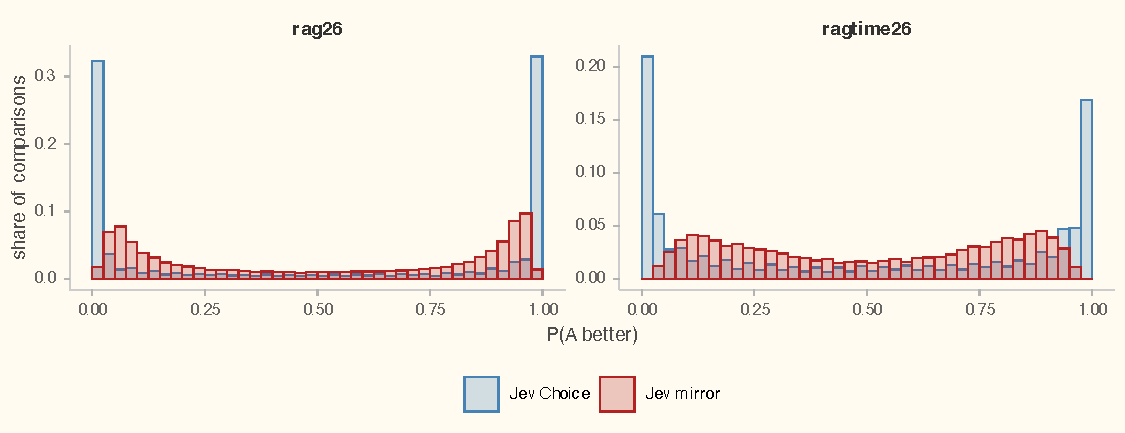
\includegraphics[width=0.9\linewidth,height=\textheight,keepaspectratio,alt={Distribution of Jev's P(A better) per comparison. Choice saturates at exactly 0 or 1 (49.8\% of comparisons on rag26, 18.5\% on ragtime26); the mirrored Noul pair never does.}]{figures_ggplot/f01_probability_distribution.pdf}
\caption{Distribution of Jev's P(A better) per comparison. Choice
saturates at exactly 0 or 1 (49.8\% of comparisons on rag26, 18.5\% on
ragtime26); the mirrored Noul pair never does.}\label{fig:f01}
\end{figure}

\begin{figure}
\centering
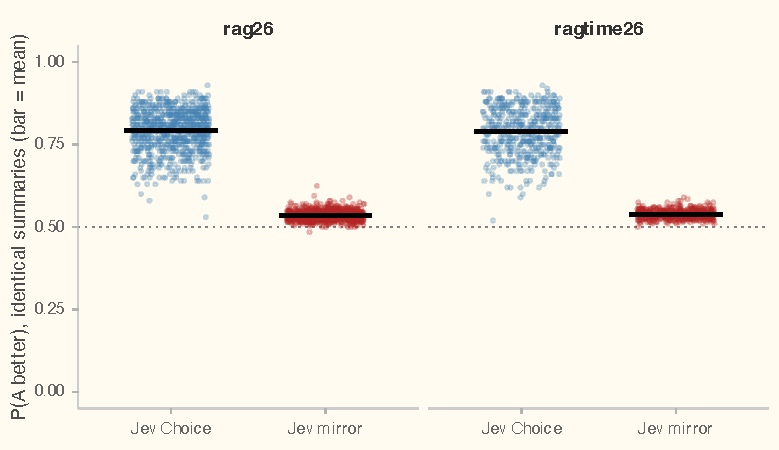
\includegraphics[width=0.55\linewidth,height=\textheight,keepaspectratio,alt={The same summary in both slots. Choice gives P(A)  0.79 on both datasets; the mirror gives 0.535 / 0.539.}]{figures_ggplot/f03_identical_summaries.pdf}
\caption{The same summary in both slots. Choice gives P(A)
\ensuremath{\approx} 0.79 on both datasets; the mirror gives 0.535 /
0.539.}\label{fig:f03}
\end{figure}

\begin{figure}
\centering
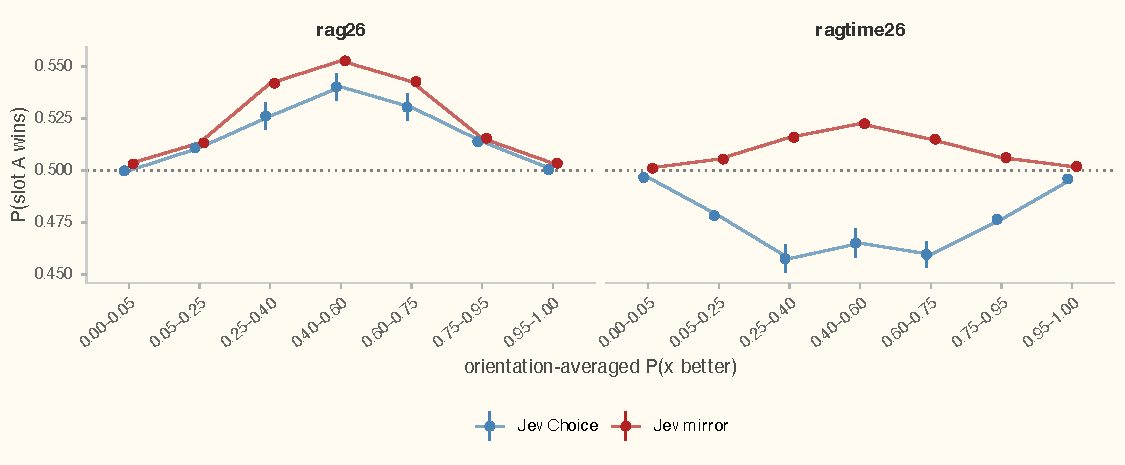
\includegraphics[width=0.8\linewidth,height=\textheight,keepaspectratio,alt={P(slot A wins) against how close the pair is, for pairs judged in both orientations (95\% CI over pairs). On close pairs (0.4--0.6), Choice favours slot A on rag26 (0.540) and slot B on ragtime26 (0.465); the mirror sits at 0.553 / 0.522.}]{figures_ggplot/f02_position_bias.pdf}
\caption{P(slot A wins) against how close the pair is, for pairs judged
in both orientations (95\% CI over pairs). On close pairs (0.4--0.6),
Choice favours slot A on rag26 (0.540) and slot B on ragtime26 (0.465);
the mirror sits at 0.553 / 0.522.}\label{fig:f02}
\end{figure}

\begin{figure}
\centering
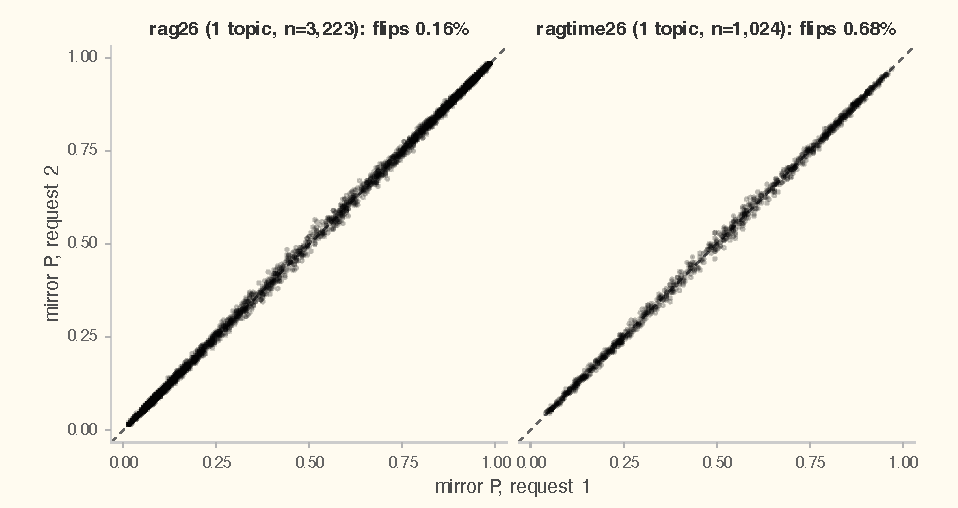
\includegraphics[width=0.7\linewidth,height=\textheight,keepaspectratio,alt={Identical mirror requests sent twice, one window topic per dataset (rag2026-3, 2003): winner flips 0.16\% / 0.68\%.}]{figures_ggplot/f13_determinism.pdf}
\caption{Identical mirror requests sent twice, one window topic per
dataset (rag2026-3, 2003): winner flips 0.16\% / 0.68\%.}\label{fig:f13}
\end{figure}

\subsubsection{4.5 Question wording}\label{question-wording}

\textbf{Prompt variants} (Figure~\ref{fig:f05}). Four Choice wordings
were asked in one request on all window topics (single orientation,
hashed):

\begin{itemize}
\tightlist
\item
  \passthrough{\lstinline!better\_summary!}, the control;
\item
  \passthrough{\lstinline!length\_neutral!};
\item
  \passthrough{\lstinline!needs\_coverage!};
\item
  \passthrough{\lstinline!precision!}.
\end{itemize}

\begin{longtable}[]{@{}
  >{\raggedright\arraybackslash}p{(\linewidth - 8\tabcolsep) * \real{0.1522}}
  >{\raggedright\arraybackslash}p{(\linewidth - 8\tabcolsep) * \real{0.1449}}
  >{\raggedright\arraybackslash}p{(\linewidth - 8\tabcolsep) * \real{0.1739}}
  >{\raggedright\arraybackslash}p{(\linewidth - 8\tabcolsep) * \real{0.2681}}
  >{\raggedright\arraybackslash}p{(\linewidth - 8\tabcolsep) * \real{0.2609}}@{}}
\toprule\noalign{}
\begin{minipage}[b]{\linewidth}\raggedright
Question
\end{minipage} & \begin{minipage}[b]{\linewidth}\raggedright
rag26 P(longer wins)
\end{minipage} & \begin{minipage}[b]{\linewidth}\raggedright
ragtime26 P(longer wins)
\end{minipage} & \begin{minipage}[b]{\linewidth}\raggedright
Ranking vs control, rag26 / ragtime26
\end{minipage} & \begin{minipage}[b]{\linewidth}\raggedright
Pair decisions agreeing with control
\end{minipage} \\
\midrule\noalign{}
\endhead
\bottomrule\noalign{}
\endlastfoot
better\_summary & 0.701 & 0.489 & --- & --- \\
length\_neutral & 0.669 & 0.450 & 0.984 / 0.957 & 95.4\% / 93.4\% \\
needs\_coverage & 0.701 & 0.499 & 0.992 / 0.944 & 96.7\% / 91.6\% \\
precision & 0.673 & 0.439 & 0.982 / 0.938 & 95.1\% / 91.0\% \\
\end{longtable}

Rewording changes 3--9\% of pair decisions but doesn't significantly
impact the ranking.

\textbf{Depth-proportionate wording} (Figure~\ref{fig:f07}). The
submitted question adds one clause to the
\passthrough{\lstinline!better!} question: ``\ldots considering
relevance, completeness, \textbf{depth proportionate to what the query
asks for (thorough when the query is broad or multi-part, brief and
direct when it is narrow)}, and how well its claims are grounded?''

Neither dataset has genuinely narrow needs, so we changed the request
instead.

\begin{itemize}
\tightlist
\item
  \textbf{Two framings of the same pairs.} The \emph{same} report pairs
  were judged under the original broad topic and under a narrow framing:
  one sub-question written from that topic's own text.
\item
  \textbf{Both pairs in each request.} Both mirrored pairs
  (\passthrough{\lstinline!better!} and
  \passthrough{\lstinline!proportionate!}) were asked in every request.
\item
  \textbf{Measure.} The difference-in-differences (DiD) of the
  broad\ensuremath{\rightarrow}narrow change in P(longer wins),
  proportionate minus \passthrough{\lstinline!better!}. A negative value
  means proportionate moves further toward shorter answers when the
  request narrows.
\end{itemize}

\begin{longtable}[]{@{}
  >{\raggedright\arraybackslash}p{(\linewidth - 4\tabcolsep) * \real{0.5161}}
  >{\raggedright\arraybackslash}p{(\linewidth - 4\tabcolsep) * \real{0.2419}}
  >{\raggedright\arraybackslash}p{(\linewidth - 4\tabcolsep) * \real{0.2419}}@{}}
\toprule\noalign{}
\begin{minipage}[b]{\linewidth}\raggedright
\end{minipage} & \begin{minipage}[b]{\linewidth}\raggedright
rag26
\end{minipage} & \begin{minipage}[b]{\linewidth}\raggedright
ragtime26
\end{minipage} \\
\midrule\noalign{}
\endhead
\bottomrule\noalign{}
\endlastfoot
\passthrough{\lstinline!better!}: P(longer), broad
\ensuremath{\rightarrow} narrow & 0.672 \ensuremath{\rightarrow} 0.640 &
0.486 \ensuremath{\rightarrow} 0.477 \\
\passthrough{\lstinline!proportionate!}: P(longer), broad
\ensuremath{\rightarrow} narrow & 0.676 \ensuremath{\rightarrow} 0.612 &
0.487 \ensuremath{\rightarrow} 0.461 \\
\textbf{DiD, pooled} & \textbf{-0.032} & \textbf{-0.016} \\
Topics with DiD \textless{} 0 & \textbf{10 / 10} (-0.015 to -0.053) &
\textbf{10 / 10} (-0.008 to -0.027) \\
Winner differs from \passthrough{\lstinline!better!}, broad framing &
0.96\% & 1.53\% \\
\end{longtable}

\begin{itemize}
\tightlist
\item
  \textbf{On the original requests,} proportionate judges like
  \passthrough{\lstinline!better!}.
\item
  \textbf{On narrowed requests,} it moves toward shorter answers about
  twice as much as \passthrough{\lstinline!better!} (rag26) or nearly
  three times as much (ragtime26).
\item
  \textbf{Caveat.} The narrow requests are synthetic: the reports were
  written for the broad request.
\end{itemize}

\begin{figure}
\centering
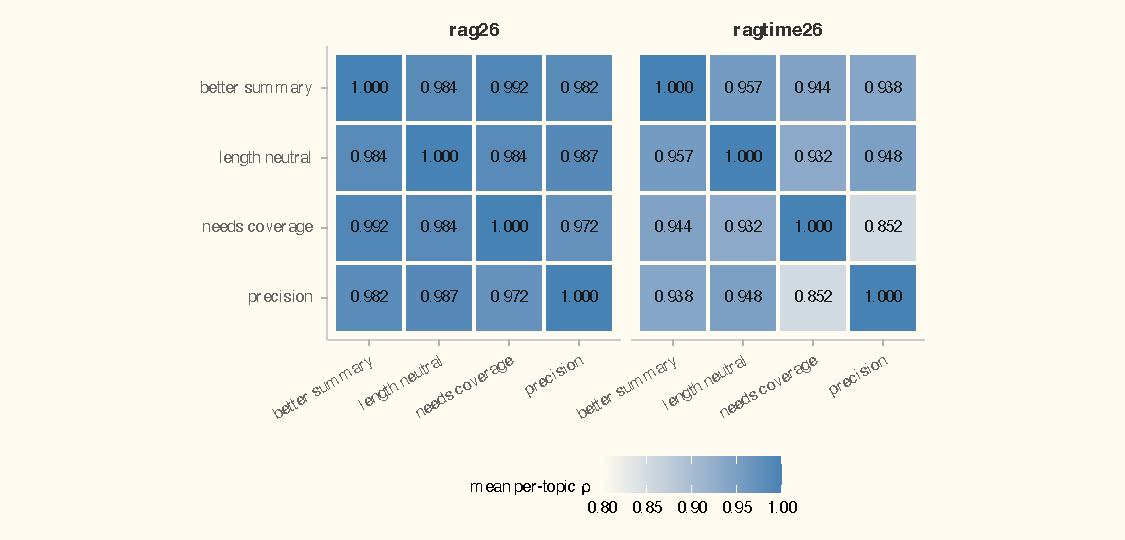
\includegraphics[width=0.85\linewidth,height=\textheight,keepaspectratio,alt={Ranking agreement between four question wordings: mean over window topics of the Spearman correlation of per-topic win rates.}]{figures_ggplot/f05_prompt_agreement.pdf}
\caption{Ranking agreement between four question wordings: mean over
window topics of the Spearman correlation of per-topic win
rates.}\label{fig:f05}
\end{figure}

\begin{figure}
\centering
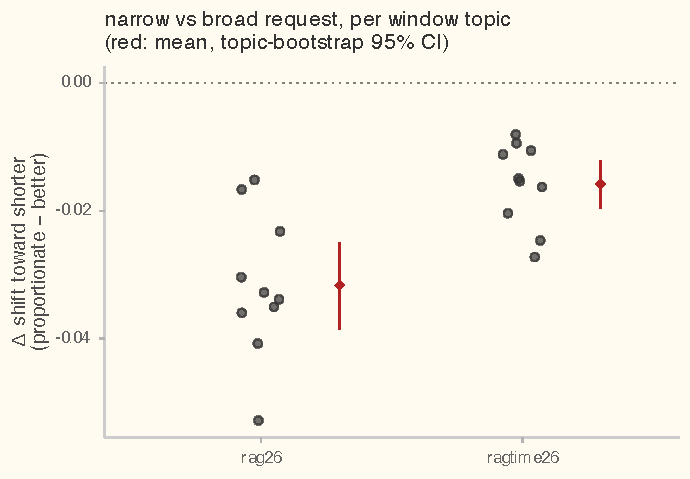
\includegraphics[width=0.6\linewidth,height=\textheight,keepaspectratio,alt={Depth-proportionate wording: per window topic, how much further the proportionate question moves toward shorter answers than better when the request is narrowed (difference-in-differences). Negative on 10/10 topics of each dataset; mean -0.032 / -0.016 with topic-bootstrap 95\% CI.}]{figures_ggplot/f07_broad_narrow.pdf}
\caption{Depth-proportionate wording: per window topic, how much further
the proportionate question moves toward shorter answers than
\passthrough{\lstinline!better!} when the request is narrowed
(difference-in-differences). Negative on 10/10 topics of each dataset;
mean -0.032 / -0.016 with topic-bootstrap 95\% CI.}\label{fig:f07}
\end{figure}

\subsubsection{4.6 Length and padding}\label{length-and-padding}

During early experiments on rag26, we found strong correlations with
longer summaries being chosen as the preferred answer by the LLM. This
section explores experiments on this hypothesis. The results show that
length is not a strong indicator of preference.

\textbf{Natural length dependence is dataset-specific}
(Figure~\ref{fig:f04}). On rag26, longer reports win (Choice P(longer) =
0.700; 0.865 when one report is at least twice as long). On ragtime26
they don't (0.488), and within topics longer reports rank slightly
lower. Every judge we ran shows the same pattern.

\textbf{Controlled padding test} (Figure~\ref{fig:f06}). Design:

\begin{itemize}
\tightlist
\item
  \textbf{Targets.} On each topic, 16 mid-ranked target runs (win rate
  0.25--0.75), giving 160 targets per dataset.
\item
  \textbf{Opponents.} Each target was judged against 8 fixed cross-team
  opponents spread over the ranking, in both orientations.
\item
  \textbf{Variants.} Each target was rewritten into five variants.
  Padding sentences were interleaved at seeded random positions, not
  appended.

  \begin{itemize}
  \tightlist
  \item
    pad\_repeat: the report's own sentences repeated
    (+\ensuremath{\approx}50\% words);
  \item
    pad\_generic: topic-agnostic filler;
  \item
    pad\_offtopic: sentences from another window topic;
  \item
    pad\_relevant: unseen sentences from the topic's strongest run of
    another team (a positive control);
  \item
    truncate: the last third of sentences removed.
  \end{itemize}
\item
  \textbf{Measure.} \ensuremath{\Delta}P is the mean change in
  orientation-averaged P(target wins) from the original, with a 95\% CI
  bootstrapped over targets.
\end{itemize}

\begin{longtable}[]{@{}
  >{\raggedright\arraybackslash}p{(\linewidth - 10\tabcolsep) * \real{0.1860}}
  >{\raggedright\arraybackslash}p{(\linewidth - 10\tabcolsep) * \real{0.0543}}
  >{\raggedright\arraybackslash}p{(\linewidth - 10\tabcolsep) * \real{0.2093}}
  >{\raggedright\arraybackslash}p{(\linewidth - 10\tabcolsep) * \real{0.1550}}
  >{\raggedright\arraybackslash}p{(\linewidth - 10\tabcolsep) * \real{0.2093}}
  >{\raggedright\arraybackslash}p{(\linewidth - 10\tabcolsep) * \real{0.1860}}@{}}
\toprule\noalign{}
\begin{minipage}[b]{\linewidth}\raggedright
Variant
\end{minipage} & \begin{minipage}[b]{\linewidth}\raggedright
Words \ensuremath{\times}
\end{minipage} & \begin{minipage}[b]{\linewidth}\raggedright
rag26 \ensuremath{\Delta}P {[}95\% CI{]}
\end{minipage} & \begin{minipage}[b]{\linewidth}\raggedright
rag26 targets \ensuremath{\Delta}P \textgreater{} 0
\end{minipage} & \begin{minipage}[b]{\linewidth}\raggedright
ragtime26 \ensuremath{\Delta}P {[}95\% CI{]}
\end{minipage} & \begin{minipage}[b]{\linewidth}\raggedright
ragtime26 targets \ensuremath{\Delta}P \textgreater{} 0
\end{minipage} \\
\midrule\noalign{}
\endhead
\bottomrule\noalign{}
\endlastfoot
pad\_repeat & 1.53 & -0.048 {[}-0.053, -0.044{]} & 1/160 & -0.074
{[}-0.080, -0.069{]} & 1/160 \\
pad\_generic & 1.51 & -0.095 {[}-0.102, -0.088{]} & 0/160 & -0.135
{[}-0.144, -0.125{]} & 1/160 \\
pad\_offtopic & 1.53 & -0.196 {[}-0.209, -0.183{]} & 0/160 & -0.258
{[}-0.271, -0.245{]} & 0/160 \\
\textbf{pad\_relevant} & 1.53 & \textbf{+0.179} {[}+0.170, +0.188{]} &
160/160 & \textbf{+0.098} {[}+0.088, +0.107{]} & 155/160 \\
truncate & 0.67 & -0.081 {[}-0.088, -0.072{]} & 2/160 & -0.078
{[}-0.088, -0.068{]} & 16/160 \\
\end{longtable}

(Submitted pairwise form, all 10 window topics.)

\textbf{Gemini baseline on the first 3 window topics.}

\begin{longtable}[]{@{}
  >{\raggedright\arraybackslash}p{(\linewidth - 4\tabcolsep) * \real{0.2500}}
  >{\raggedright\arraybackslash}p{(\linewidth - 4\tabcolsep) * \real{0.3750}}
  >{\raggedright\arraybackslash}p{(\linewidth - 4\tabcolsep) * \real{0.3750}}@{}}
\toprule\noalign{}
\begin{minipage}[b]{\linewidth}\raggedright
Variant
\end{minipage} & \begin{minipage}[b]{\linewidth}\raggedright
rag26 \ensuremath{\Delta}P {[}95\% CI{]}
\end{minipage} & \begin{minipage}[b]{\linewidth}\raggedright
ragtime26 \ensuremath{\Delta}P {[}95\% CI{]}
\end{minipage} \\
\midrule\noalign{}
\endhead
\bottomrule\noalign{}
\endlastfoot
pad\_repeat & -0.132 {[}-0.160, -0.104{]} & -0.203 {[}-0.249,
-0.160{]} \\
pad\_generic & -0.104 {[}-0.130, -0.079{]} & -0.186 {[}-0.224,
-0.150{]} \\
pad\_offtopic & -0.206 {[}-0.250, -0.165{]} & -0.309 {[}-0.368,
-0.250{]} \\
pad\_relevant & \textbf{+0.104} {[}+0.070, +0.138{]} & \textbf{-0.117}
{[}-0.151, -0.085{]} \\
truncate & -0.078 {[}-0.107, -0.049{]} & -0.152 {[}-0.195, -0.113{]} \\
\end{longtable}

\begin{itemize}
\tightlist
\item
  \textbf{Jev.} It penalises all three uninformative paddings and
  credits relevant content on every topic of both datasets.
\item
  \textbf{Gemini on ragtime26.} It penalises any added text, relevant or
  not. This test can't tell whether Gemini reads the splice as
  disruption or doesn't credit coverage.
\item
  \textbf{Not tested.} Subtle on-topic verbosity: restatement or hedging
  with no new facts.
\end{itemize}

\begin{figure}
\centering
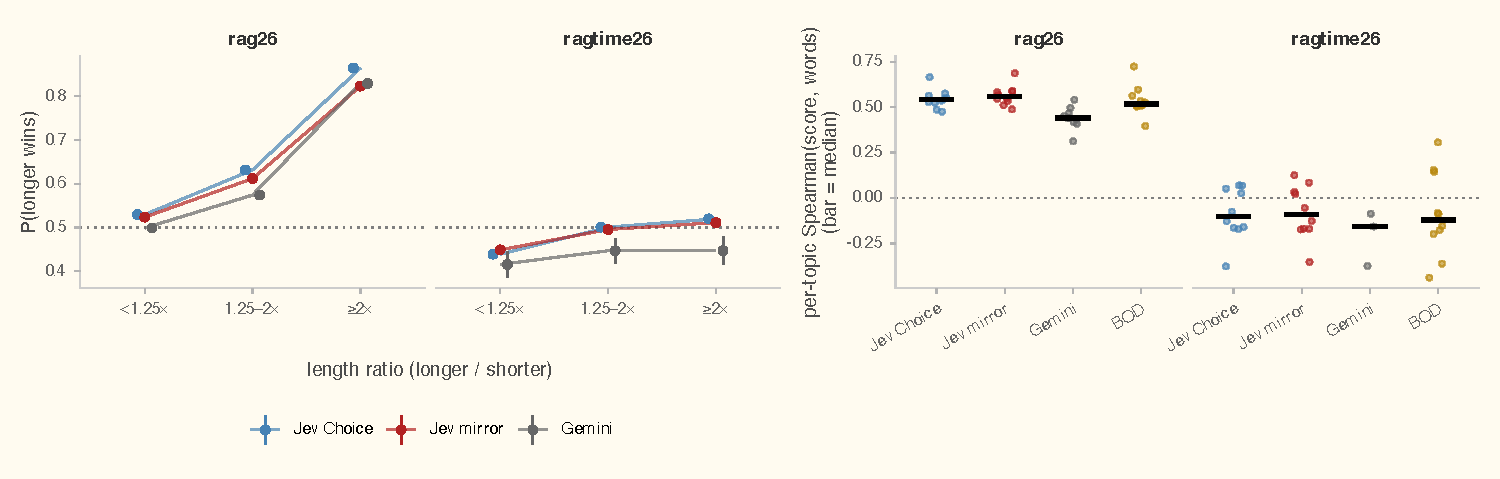
\includegraphics[width=1\linewidth,height=\textheight,keepaspectratio,alt={Left and centre: P(longer report wins) by length ratio (95\% CI over comparisons). Right: per-topic Spearman between score and word count (bar = median). On rag26 longer reports win under every judge; on ragtime26 they don't. Gemini covers 3 ragtime26 topics.}]{figures_ggplot/f04_length.pdf}
\caption{Left and centre: P(longer report wins) by length ratio (95\% CI
over comparisons). Right: per-topic Spearman between score and word
count (bar = median). On rag26 longer reports win under every judge; on
ragtime26 they don't. Gemini covers 3 ragtime26 topics.}\label{fig:f04}
\end{figure}

\begin{figure}
\centering
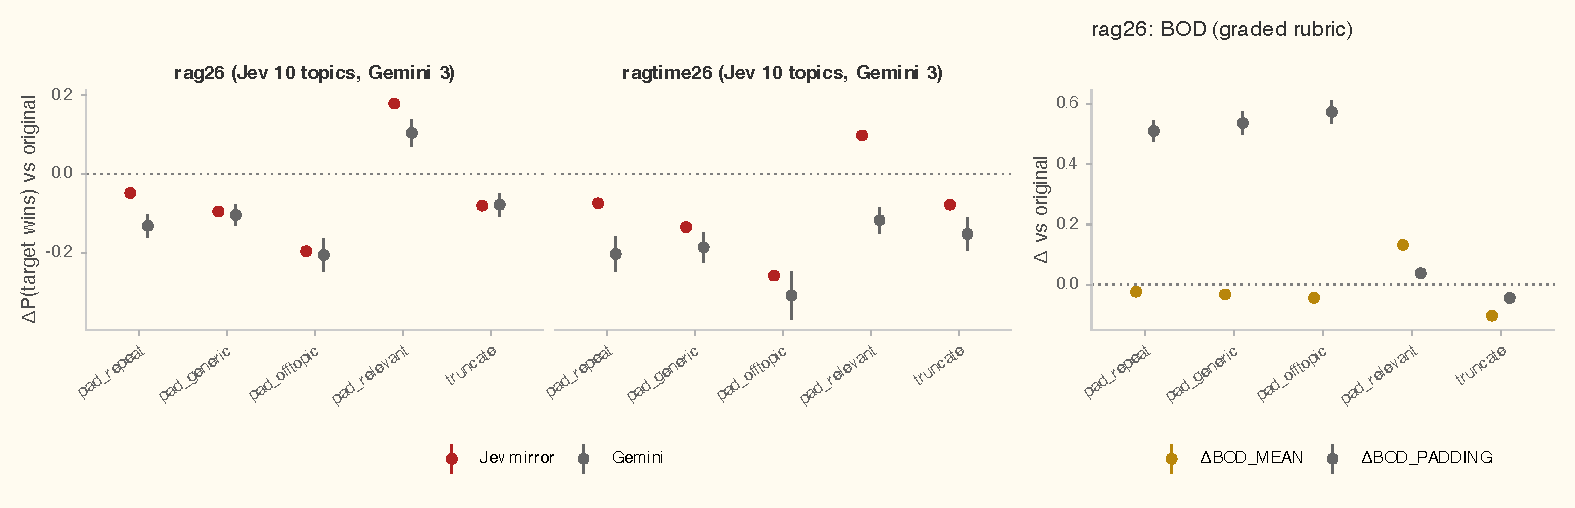
\includegraphics[width=1\linewidth,height=\textheight,keepaspectratio,alt={Controlled padding: change from the unmodified report (95\% CI over targets). Left and centre: pairwise judges, P(target wins); Jev mirror over 10 topics, Gemini over 3. Right: BOD on rag26, BOD\_MEAN and BOD\_PADDING. Uninformative padding lowers scores; relevant padding raises them, except Gemini on ragtime26.}]{figures_ggplot/f06_padding.pdf}
\caption{Controlled padding: change from the unmodified report (95\% CI
over targets). Left and centre: pairwise judges,
\ensuremath{\Delta}P(target wins); Jev mirror over 10 topics, Gemini
over 3. Right: BOD on rag26, \ensuremath{\Delta}BOD\_MEAN and
\ensuremath{\Delta}BOD\_PADDING. Uninformative padding lowers scores;
relevant padding raises them, except Gemini on
ragtime26.}\label{fig:f06}
\end{figure}

\subsubsection{4.7 Pre-registered
decisions}\label{pre-registered-decisions}

\begin{longtable}[]{@{}
  >{\raggedright\arraybackslash}p{(\linewidth - 6\tabcolsep) * \real{0.0240}}
  >{\raggedright\arraybackslash}p{(\linewidth - 6\tabcolsep) * \real{0.6048}}
  >{\raggedright\arraybackslash}p{(\linewidth - 6\tabcolsep) * \real{0.1856}}
  >{\raggedright\arraybackslash}p{(\linewidth - 6\tabcolsep) * \real{0.1856}}@{}}
\toprule\noalign{}
\begin{minipage}[b]{\linewidth}\raggedright
\#
\end{minipage} & \begin{minipage}[b]{\linewidth}\raggedright
Criterion (written beforehand)
\end{minipage} & \begin{minipage}[b]{\linewidth}\raggedright
rag26 (decision)
\end{minipage} & \begin{minipage}[b]{\linewidth}\raggedright
ragtime26 (confirmation)
\end{minipage} \\
\midrule\noalign{}
\endhead
\bottomrule\noalign{}
\endlastfoot
1 & Proportionate DiD \textless{} 0 on \ensuremath{\geq} 7/10 topics,
topic-bootstrap CI excludes 0 & Pass: 10/10, -0.032 & Confirmed: 10/10,
-0.016 \\
2 & Identical summaries within {[}0.40, 0.60{]} & Pass: 0.535 &
Confirmed: 0.539 \\
3 & Drop one orientation only if close-pair slot bias is non-significant
and ties are within {[}0.45, 0.55{]} & Keep both: 0.553 {[}0.547,
0.559{]} & Confirmed: 0.523 {[}0.514, 0.532{]} \\
4 & Uninformative padding \ensuremath{\Delta}P \textless{} 0 (CI
excludes 0); relevant \ensuremath{\Delta}P \textgreater{} 0 & Pass &
Confirmed \\
5 & Reopen Choice only if the mirror flips \textgreater{} 2\% of winners
or \ensuremath{\rho} vs Choice \textless{} 0.95 & Not reopened: 0.155\%,
\ensuremath{\rho} 0.998 & Confirmed: 0.684\%, \ensuremath{\rho} 0.998 \\
\end{longtable}

Decision 3 uses topic-bootstrap 95\% CIs on P(slot A wins) for close
pairs. The bias appeared on every topic: 0.537--0.572 on rag26 and
0.503--0.549 on ragtime26.

\subsubsection{4.8 Submitted configuration and full
runs}\label{submitted-configuration-and-full-runs}

\begin{itemize}
\tightlist
\item
  \textbf{Questions.} \passthrough{\lstinline!noul\_a\_proportionate!}
  and \passthrough{\lstinline!noul\_b\_proportionate!} in one request,
  scored by their mirror average.
\item
  \textbf{Coverage.} Both orientations of every cross-team pair, on
  every topic.
\end{itemize}

\begin{longtable}[]{@{}lll@{}}
\toprule\noalign{}
& ragtime26 & rag26 \\
\midrule\noalign{}
\endhead
\bottomrule\noalign{}
\endlastfoot
Comparisons (ordered) & 210,418, all valid & 760,886, all valid \\
Unique calls & 196,958 & 703,536 \\
Cost & \$18.95 & \$74.89 \\
Wall-clock & 3.0 h & 11.1 h \\
\end{longtable}

\textbf{Window diagnostics of the full runs} (Figures \ref{fig:f02},
\ref{fig:f04}, \ref{fig:f12}):

\begin{longtable}[]{@{}
  >{\raggedright\arraybackslash}p{(\linewidth - 4\tabcolsep) * \real{0.6142}}
  >{\raggedright\arraybackslash}p{(\linewidth - 4\tabcolsep) * \real{0.1969}}
  >{\raggedright\arraybackslash}p{(\linewidth - 4\tabcolsep) * \real{0.1890}}@{}}
\toprule\noalign{}
\begin{minipage}[b]{\linewidth}\raggedright
Metric
\end{minipage} & \begin{minipage}[b]{\linewidth}\raggedright
rag26
\end{minipage} & \begin{minipage}[b]{\linewidth}\raggedright
ragtime26
\end{minipage} \\
\midrule\noalign{}
\endhead
\bottomrule\noalign{}
\endlastfoot
Split-half reliability & 0.974 {[}0.960, 0.982{]} & 0.948 {[}0.915,
0.970{]} \\
Board \ensuremath{\rho} / Kendall vs Gemini & 0.974 / 0.866 (10 topics)
& 0.939 / 0.818 (3 topics) \\
P(longer wins); per-topic \ensuremath{\rho}(win rate, words), median &
0.675; +0.558 & 0.486; -0.090 \\
P(slot A wins): all / close pairs & 0.520 / 0.553 & 0.511 / 0.523 \\
Flagged near-ties & 0.84\% & 2.80\% \\
\end{longtable}

\begin{center}\rule{0.5\linewidth}{0.5pt}\end{center}

\subsection{5. Judge 2: bag-of-decisions graded rubric
(BOD)}\label{judge-2-bag-of-decisions-graded-rubric-bod}

\subsubsection{5.1 Design}\label{design}

This judge adapts a ``Bag of Decisions (BOD) Reranker'' (well outlined
in a post by Doug Turnbull). There, an LLM writes yes/no criteria per
query, Jev answers them all in one request, and the score is the sum of
P(yes). We change three things: the number of questions varies by topic,
the questions are graded 0--3, and the grades are stored and tallied
afterwards.

\begin{enumerate}
\def\labelenumi{\arabic{enumi}.}
\tightlist
\item
  \textbf{Rubric.}

  \begin{itemize}
  \tightlist
  \item
    Gemini 2.5 Flash Lite at temperature 0 writes 5--15 ``Does the
    answer \ldots?'' questions per topic, sized to how many distinct
    parts the need has.
  \item
    It sees the topic text only (query, problem statement, background),
    never a response.
  \item
    Near-duplicates are dropped (token Jaccard \ensuremath{\geq} 0.8).
  \item
    The prompt is in Appendix A.2. It was settled on kiddie only, before
    any 2026 data was read. Its first version produced persona questions
    such as ``Does the answer acknowledge the child's interest\ldots?'';
    the final version allows content questions only.
  \end{itemize}
\item
  \textbf{Grading.}

  \begin{itemize}
  \tightlist
  \item
    One Jev request per (run, topic). The state is the topic fields plus
    the answer.
  \item
    Each rubric question is a 4-option Choice with anchored grades:

    \begin{itemize}
    \tightlist
    \item
      0: not addressed;
    \item
      1: mentioned without substance;
    \item
      2: partially answered;
    \item
      3: fully answered with specific, accurate detail.
    \end{itemize}
  \item
    The same request carries a Noul padding question as a diagnostic.
  \end{itemize}
\item
  \textbf{Scoring.}

  \begin{itemize}
  \tightlist
  \item
    Each question scores its \textbf{expected grade}
    \ensuremath{\sum_g P(g)\cdot g} / 3, from the probabilities, as in
    G-Eval.
  \item
    The overall score is the mean over the topic's questions, then the
    mean over topics.
  \end{itemize}
\end{enumerate}

\begin{longtable}[]{@{}
  >{\raggedright\arraybackslash}p{(\linewidth - 2\tabcolsep) * \real{0.2521}}
  >{\raggedright\arraybackslash}p{(\linewidth - 2\tabcolsep) * \real{0.7479}}@{}}
\toprule\noalign{}
\begin{minipage}[b]{\linewidth}\raggedright
Measure
\end{minipage} & \begin{minipage}[b]{\linewidth}\raggedright
Definition
\end{minipage} \\
\midrule\noalign{}
\endhead
\bottomrule\noalign{}
\endlastfoot
\passthrough{\lstinline!BOD\_MEAN!} (primary) & mean expected grade over
the topic's questions, divided by 3 \\
\passthrough{\lstinline!BOD\_COVERAGE!} & fraction of questions with
P(grade \ensuremath{\geq} 2) \textgreater{} 0.5 \\
\passthrough{\lstinline!BOD\_FULL!} & fraction of questions with P(grade
= 3) \textgreater{} 0.5 \\
\passthrough{\lstinline!BOD\_PADDING!} & P(yes) that the answer has
substantial off-topic, repeated or generic filler (diagnostic) \\
\passthrough{\lstinline!BOD\_QUESTIONS!} & number of rubric questions \\
\end{longtable}

Each answer is scored on its own, so a topic needs O(runs) calls instead
of O(runs²).

\subsubsection{5.2 Window results}\label{window-results}

We saw strong correlation with pairwise, justifying the significant
reduction in cost without sacrificing perceived accuracy.

\begin{longtable}[]{@{}
  >{\raggedright\arraybackslash}p{(\linewidth - 4\tabcolsep) * \real{0.5000}}
  >{\raggedright\arraybackslash}p{(\linewidth - 4\tabcolsep) * \real{0.2500}}
  >{\raggedright\arraybackslash}p{(\linewidth - 4\tabcolsep) * \real{0.2500}}@{}}
\toprule\noalign{}
\begin{minipage}[b]{\linewidth}\raggedright
\end{minipage} & \begin{minipage}[b]{\linewidth}\raggedright
rag26 window
\end{minipage} & \begin{minipage}[b]{\linewidth}\raggedright
ragtime26 window
\end{minipage} \\
\midrule\noalign{}
\endhead
\bottomrule\noalign{}
\endlastfoot
Answers / cost & 828 / \$0.09 & 490 / \$0.05 \\
Questions per topic & 5--13 (mean 9.0) & 6--10 \\
BOD\_MEAN p10 / p50 / p90 & 0.420 / 0.756 / 0.983 & 0.514 / 0.710 /
0.894 \\
Most likely grade 0 / 1 / 2 / 3 & 8.2\% / 9.2\% / 40.3\% / 42.3\% &
8.4\% / 7.8\% / 46.4\% / 37.5\% \\
\textbar E{[}g{]} - most likely grade\textbar{} \textgreater{} 0.25 &
26.9\% of questions & 37.7\% \\
Split-half (5 vs 5) & 0.969 {[}0.956, 0.979{]} & 0.854 {[}0.789,
0.914{]} \\
Per-topic \ensuremath{\rho}(BOD\_MEAN, words), median & 0.518 &
-0.120 \\
Board \ensuremath{\rho} vs pairwise judge & \textbf{0.990} (Kendall
0.919) & 0.918 (Figure~\ref{fig:f08}) \\
Board \ensuremath{\rho} vs Gemini & 0.972 (7 topics) & --- \\
\end{longtable}

\begin{itemize}
\tightlist
\item
  \textbf{Probabilities.} The expected grade differs meaningfully from
  the most likely grade on a quarter to a third of questions, so here
  the probabilities carry information (Figure~\ref{fig:f09}).
\item
  \textbf{Ceiling.} Grades saturate near 3 on rag26, which compresses
  the top of the board.
\end{itemize}

\begin{figure}
\centering
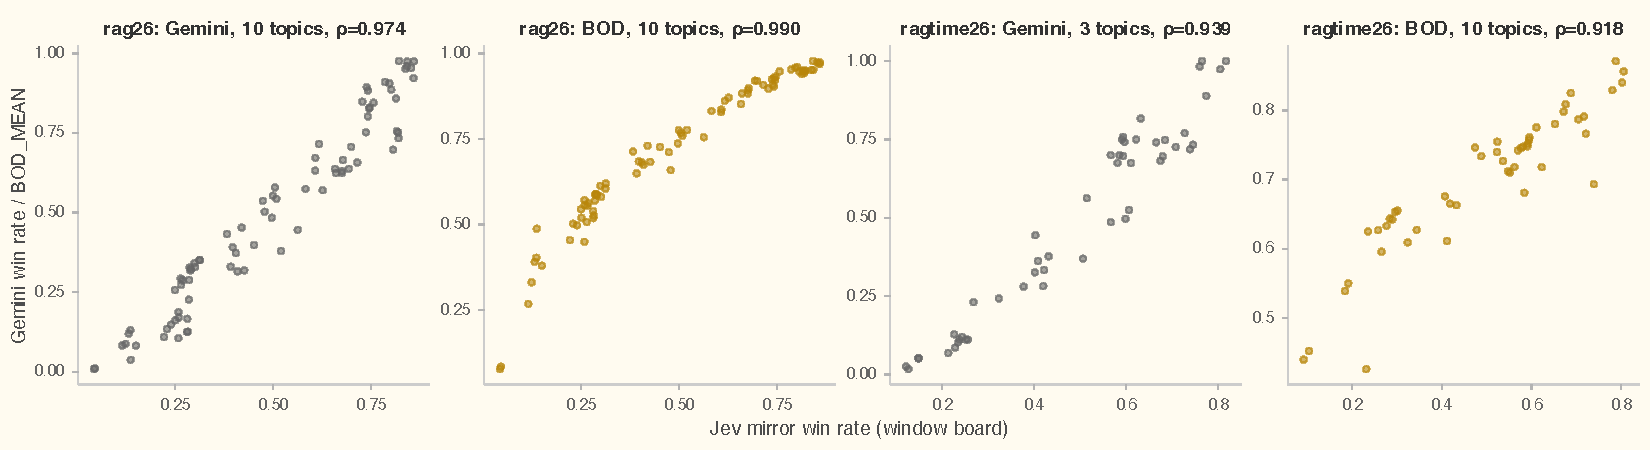
\includegraphics[width=1\linewidth,height=\textheight,keepaspectratio,alt={Run boards on the window. Jev mirror vs Gemini ( 0.974 on 10 rag26 topics, 0.939 on 3 ragtime26 topics), and BOD vs Jev mirror ( 0.990 rag26, 0.918 ragtime26).}]{figures_ggplot/f08_judge_agreement.pdf}
\caption{Run boards on the window. Jev mirror vs Gemini
(\ensuremath{\rho} 0.974 on 10 rag26 topics, 0.939 on 3 ragtime26
topics), and BOD vs Jev mirror (\ensuremath{\rho} 0.990 rag26, 0.918
ragtime26).}\label{fig:f08}
\end{figure}

\begin{figure}
\centering
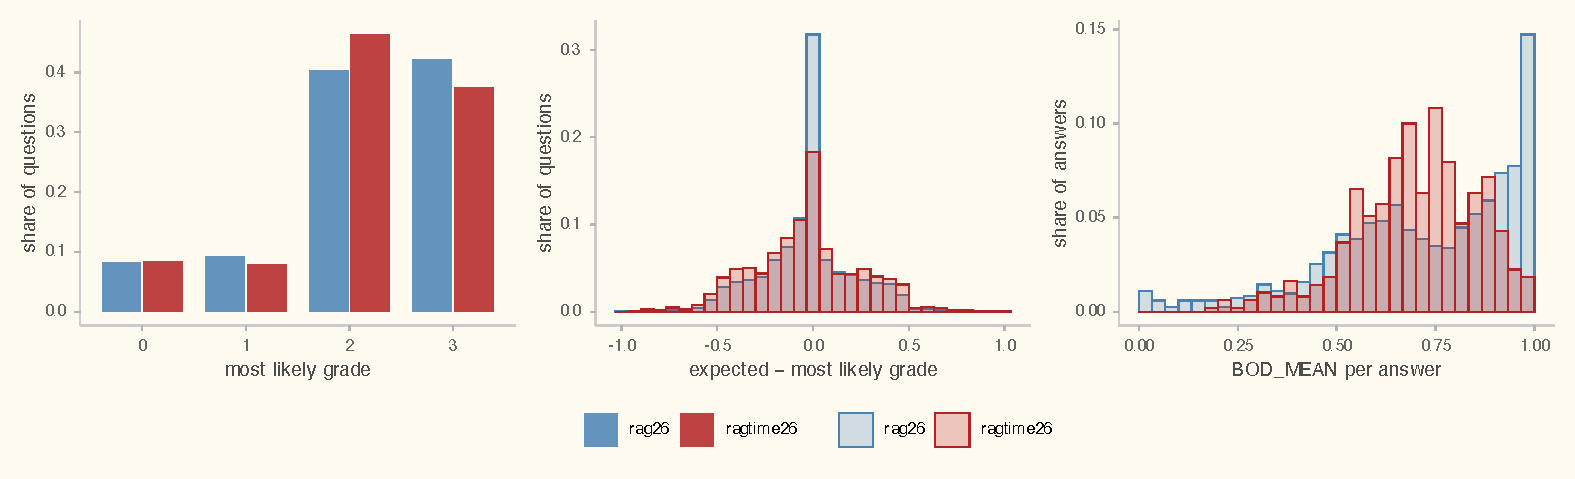
\includegraphics[width=1\linewidth,height=\textheight,keepaspectratio,alt={BOD grades on the window: most likely grade per question; expected minus most likely grade (\textbar\textbar{} \textgreater{} 0.25 for 26.9\% / 37.7\% of questions); BOD\_MEAN per answer, with the rag26 ceiling.}]{figures_ggplot/f09_bod_grades.pdf}
\caption{BOD grades on the window: most likely grade per question;
expected minus most likely grade (\textbar{}\ensuremath{\cdot}\textbar{}
\textgreater{} 0.25 for 26.9\% / 37.7\% of questions); BOD\_MEAN per
answer, with the rag26 ceiling.}\label{fig:f09}
\end{figure}

\subsubsection{5.3 Padding test (rag26
window)}\label{padding-test-rag26-window}

The design is that of §4.6, with each variant graded on its own (160
targets \ensuremath{\times} 6 variants). The criteria were written into
the analysis script before the run.

\begin{longtable}[]{@{}
  >{\raggedright\arraybackslash}p{(\linewidth - 6\tabcolsep) * \real{0.2400}}
  >{\raggedright\arraybackslash}p{(\linewidth - 6\tabcolsep) * \real{0.0933}}
  >{\raggedright\arraybackslash}p{(\linewidth - 6\tabcolsep) * \real{0.3600}}
  >{\raggedright\arraybackslash}p{(\linewidth - 6\tabcolsep) * \real{0.3067}}@{}}
\toprule\noalign{}
\begin{minipage}[b]{\linewidth}\raggedright
Variant
\end{minipage} & \begin{minipage}[b]{\linewidth}\raggedright
Words \ensuremath{\times}
\end{minipage} & \begin{minipage}[b]{\linewidth}\raggedright
\ensuremath{\Delta}BOD\_MEAN {[}95\% CI{]}
\end{minipage} & \begin{minipage}[b]{\linewidth}\raggedright
\ensuremath{\Delta}BOD\_PADDING {[}95\% CI{]}
\end{minipage} \\
\midrule\noalign{}
\endhead
\bottomrule\noalign{}
\endlastfoot
pad\_repeat & 1.52 & -0.023 {[}-0.025, -0.020{]} & +0.510 {[}+0.474,
+0.544{]} \\
pad\_generic & 1.51 & -0.032 {[}-0.035, -0.028{]} & +0.537 {[}+0.499,
+0.574{]} \\
pad\_offtopic & 1.53 & -0.043 {[}-0.047, -0.039{]} & +0.574 {[}+0.535,
+0.612{]} \\
pad\_relevant & 1.54 & \textbf{+0.132} {[}+0.121, +0.144{]} & +0.038
{[}+0.021, +0.055{]} \\
truncate & 0.67 & \textbf{-0.103} {[}-0.114, -0.092{]} & -0.044
{[}-0.061, -0.027{]} \\
\end{longtable}

Every criterion passes on each of the 10 topics individually
(Figure~\ref{fig:f06}, right).

\subsubsection{5.4 Full runs}\label{full-runs}

\begin{longtable}[]{@{}
  >{\raggedright\arraybackslash}p{(\linewidth - 4\tabcolsep) * \real{0.5652}}
  >{\raggedright\arraybackslash}p{(\linewidth - 4\tabcolsep) * \real{0.2174}}
  >{\raggedright\arraybackslash}p{(\linewidth - 4\tabcolsep) * \real{0.2174}}@{}}
\toprule\noalign{}
\begin{minipage}[b]{\linewidth}\raggedright
\end{minipage} & \begin{minipage}[b]{\linewidth}\raggedright
ragtime26
\end{minipage} & \begin{minipage}[b]{\linewidth}\raggedright
rag26
\end{minipage} \\
\midrule\noalign{}
\endhead
\bottomrule\noalign{}
\endlastfoot
Topics / runs & 103 / 49 & 119 / 83 \\
Rubric questions per topic & 5--11 (mean 7.7) & 5--15 (mean 8.4) \\
Answers graded & 5,041 / 5,041 & 9,838 / 9,838 \\
Wall-clock & 3.0 min & 8.5 min \\
\end{longtable}

Cost: \$1.31 for both datasets, including rubric generation.

\begin{center}\rule{0.5\linewidth}{0.5pt}\end{center}

\subsection{\texorpdfstring{6. Judge 3: BOD \ensuremath{\times}
Hallucination
Risk}{6. Judge 3: BOD  Hallucination Risk}}\label{judge-3-bod-hallucination-risk}

\subsubsection{6.1 Definition}\label{definition}

BOD rewards answering the rubric but doesn't check whether the answer's
claims are supported by its citations. This judge discounts each answer
by the share of its content that is unsupported \emph{and} that no other
run produced.

\textbf{Concepts.}

\begin{itemize}
\tightlist
\item
  A concept is a normalized spaCy
  \passthrough{\lstinline!en\_core\_web\_lg!} NOUN/PROPN phrase. We
  normalize by taking the lemma, lowercased.
\item
  \passthrough{\lstinline!sn!} is the answer's concept set.
\item
  \passthrough{\lstinline!hn!} is the union of the concept sets of the
  documents the answer cites.
\item
  \passthrough{\lstinline!df[t][c]!} is the number of runs whose answer
  for topic \emph{t} states concept \emph{c}.
\end{itemize}

\textbf{Measures.}

\begin{itemize}
\tightlist
\item
  \textbf{Ungrounded} concepts are \passthrough{\lstinline!sn - hn!},
  those absent from every cited document.
  \passthrough{\lstinline!UNGROUNDED\_RATE!} = \textbar sn -
  hn\textbar{} / \textbar sn\textbar{} = 1 - concept precision.
\item
  \textbf{Private-ungrounded} concepts are the ungrounded ones that no
  other run states (\passthrough{\lstinline!df!} = 1).
\item
  \passthrough{\lstinline!HALLUC\_RISK!} =
  \textbar private-ungrounded\textbar{} / \textbar sn\textbar.
\item
  \passthrough{\lstinline!BOD\_GROUNDED!} =
  \passthrough{\lstinline!BOD\_MEAN!} \ensuremath{\times} (1 -
  \passthrough{\lstinline!HALLUC\_RISK!}) per answer, then the mean over
  topics. There is no weight or threshold to set.
\item
  \textbf{Undefined risk} (no citations, no cited-document text, or no
  concepts) is set to 1. This is a policy choice.
\end{itemize}

\textbf{Relation to prior work.}

\begin{itemize}
\tightlist
\item
  The ungrounded rate is the complement of the precision side of Irwin's
  concept F1, which compares the nouns in a summary with the nouns in
  its cited sources.
\item
  The cross-run condition is our addition and is a cross-system analogue
  of SelfCheckGPT's consistency check across samples.
\item
  The measure is lexical, but needs inference against the local spaCy
  model for each cited document and answer.
\end{itemize}

\subsubsection{6.2 Pre-registered criteria and window
results}\label{pre-registered-criteria-and-window-results}

\begin{longtable}[]{@{}
  >{\raggedright\arraybackslash}p{(\linewidth - 4\tabcolsep) * \real{0.6467}}
  >{\raggedright\arraybackslash}p{(\linewidth - 4\tabcolsep) * \real{0.1467}}
  >{\raggedright\arraybackslash}p{(\linewidth - 4\tabcolsep) * \real{0.2067}}@{}}
\toprule\noalign{}
\begin{minipage}[b]{\linewidth}\raggedright
Criterion
\end{minipage} & \begin{minipage}[b]{\linewidth}\raggedright
rag26 window (dev)
\end{minipage} & \begin{minipage}[b]{\linewidth}\raggedright
ragtime26 window (confirmation)
\end{minipage} \\
\midrule\noalign{}
\endhead
\bottomrule\noalign{}
\endlastfoot
1 Pipeline: 0 new Jev calls; risk defined for \ensuremath{\geq} 99\% of
answers & 826/828: pass & 490/490: pass \\
2 Not redundant: board \ensuremath{\rho}(GROUNDED, MEAN) \textless{}
0.99 & 0.992: \textbf{fail} & 0.984: pass \\
3 Not dominant: same \ensuremath{\rho} \ensuremath{\geq} 0.70 & pass &
pass \\
4 Reliability: split-half \ensuremath{\geq} BOD\_MEAN's - 0.05 & 0.968
vs 0.969: pass & 0.820 vs 0.854: pass \\
5 Length: \textbar{}\ensuremath{\rho}(score, words)\textbar{}
\ensuremath{\leq} BOD\_MEAN's + 0.15 & +0.505 vs +0.523: pass & -0.163
vs -0.120: pass \\
6 Pool stability: half the other runs removed from
\passthrough{\lstinline!df!}, \ensuremath{\rho} \ensuremath{\geq} 0.90 &
min 0.993: pass & min 0.910: pass \\
\end{longtable}

\begin{longtable}[]{@{}
  >{\raggedright\arraybackslash}p{(\linewidth - 4\tabcolsep) * \real{0.6500}}
  >{\raggedright\arraybackslash}p{(\linewidth - 4\tabcolsep) * \real{0.1750}}
  >{\raggedright\arraybackslash}p{(\linewidth - 4\tabcolsep) * \real{0.1750}}@{}}
\toprule\noalign{}
\begin{minipage}[b]{\linewidth}\raggedright
Diagnostic (window)
\end{minipage} & \begin{minipage}[b]{\linewidth}\raggedright
rag26
\end{minipage} & \begin{minipage}[b]{\linewidth}\raggedright
ragtime26
\end{minipage} \\
\midrule\noalign{}
\endhead
\bottomrule\noalign{}
\endlastfoot
HALLUC\_RISK mean / median / p75 & 0.021 / 0.009 / 0.027 & 0.025 / 0.013
/ 0.036 \\
UNGROUNDED\_RATE mean & 0.104 & 0.140 \\
Per-topic \ensuremath{\rho}(risk, number of cited documents), median &
+0.165 & +0.131 \\
Per-topic \ensuremath{\rho}(risk, BOD\_MEAN), median & +0.331 &
+0.347 \\
\end{longtable}

\begin{itemize}
\tightlist
\item
  \textbf{Criterion 2 failed on rag26:} the discount barely changes the
  ranking. We submitted the judge anyway as a separate run, and recorded
  that decision before reading ragtime26.
\item
  \textbf{Small effect.} About four in five unsupported concepts are
  also stated by some other run, so the private share is small (Figures
  \ref{fig:f10a} and \ref{fig:f10b}).
\item
  \textbf{No sign of citation gaming.} Risk rises slightly, rather than
  falls, with the number of cited documents.
\item
  \textbf{Leans against stronger answers.} Risk correlates positively
  with BOD\_MEAN, so the discount leans slightly against the stronger
  answers. Whether those private concepts are hallucinations or useful
  detail needs assessments.
\end{itemize}

\begin{figure}
\centering
\includegraphics[width=0.5\linewidth,height=\textheight,keepaspectratio,alt={HALLUC\_RISK and UNGROUNDED\_RATE per answer (risk defined); median risk 0.009 / 0.013.}]{figures_ggplot/f10a_hallucination_risk.pdf}
\caption{HALLUC\_RISK and UNGROUNDED\_RATE per answer (risk defined);
median risk 0.009 / 0.013.}\label{fig:f10a}
\end{figure}

\begin{figure}
\centering
\includegraphics[width=0.85\linewidth,height=\textheight,keepaspectratio,alt={BOD\_GROUNDED vs BOD\_MEAN per answer. The two answers at 0 on rag26 have undefined risk (no usable citations).}]{figures_ggplot/f10b_grounded_vs_mean.pdf}
\caption{BOD\_GROUNDED vs BOD\_MEAN per answer. The two answers at 0 on
rag26 have undefined risk (no usable citations).}\label{fig:f10b}
\end{figure}

\subsubsection{6.3 Full runs}\label{full-runs-1}

\begin{longtable}[]{@{}
  >{\raggedright\arraybackslash}p{(\linewidth - 4\tabcolsep) * \real{0.7391}}
  >{\raggedright\arraybackslash}p{(\linewidth - 4\tabcolsep) * \real{0.1304}}
  >{\raggedright\arraybackslash}p{(\linewidth - 4\tabcolsep) * \real{0.1304}}@{}}
\toprule\noalign{}
\begin{minipage}[b]{\linewidth}\raggedright
\end{minipage} & \begin{minipage}[b]{\linewidth}\raggedright
ragtime26
\end{minipage} & \begin{minipage}[b]{\linewidth}\raggedright
rag26
\end{minipage} \\
\midrule\noalign{}
\endhead
\bottomrule\noalign{}
\endlastfoot
Answers graded / new Jev calls & 5,041 / 0 & 9,838 / 0 \\
Risk defined & 5,033 & 9,791 \\
Cited documents tagged & 10,394 & 61,151 \\
Wall-clock (spaCy, single process) & 10 min & 146 min \\
\end{longtable}

\begin{center}\rule{0.5\linewidth}{0.5pt}\end{center}

\subsection{7. Agreement between the submitted judges (all
topics)}\label{agreement-between-the-submitted-judges-all-topics}

Read from the submitted leaderboards' aggregate rows after submission,
for reporting only (Figure~\ref{fig:f11}).

\begin{longtable}[]{@{}
  >{\raggedright\arraybackslash}p{(\linewidth - 4\tabcolsep) * \real{0.4091}}
  >{\raggedright\arraybackslash}p{(\linewidth - 4\tabcolsep) * \real{0.2727}}
  >{\raggedright\arraybackslash}p{(\linewidth - 4\tabcolsep) * \real{0.3182}}@{}}
\toprule\noalign{}
\begin{minipage}[b]{\linewidth}\raggedright
Pair of judges
\end{minipage} & \begin{minipage}[b]{\linewidth}\raggedright
rag26 Spearman / Kendall
\end{minipage} & \begin{minipage}[b]{\linewidth}\raggedright
ragtime26 Spearman / Kendall
\end{minipage} \\
\midrule\noalign{}
\endhead
\bottomrule\noalign{}
\endlastfoot
BOD\_MEAN vs pairwise & 0.991 / 0.929 & 0.943 / 0.827 \\
BOD\_GROUNDED vs BOD\_MEAN & 0.993 / 0.952 & 0.975 / 0.884 \\
BOD\_GROUNDED vs pairwise & 0.982 / 0.890 & 0.911 / 0.765 \\
\end{longtable}

\begin{longtable}[]{@{}
  >{\raggedright\arraybackslash}p{(\linewidth - 4\tabcolsep) * \real{0.3267}}
  >{\raggedright\arraybackslash}p{(\linewidth - 4\tabcolsep) * \real{0.3366}}
  >{\raggedright\arraybackslash}p{(\linewidth - 4\tabcolsep) * \real{0.3366}}@{}}
\toprule\noalign{}
\begin{minipage}[b]{\linewidth}\raggedright
Rank movement
\end{minipage} & \begin{minipage}[b]{\linewidth}\raggedright
BOD vs pairwise: rag26 / ragtime26
\end{minipage} & \begin{minipage}[b]{\linewidth}\raggedright
GROUNDED vs BOD: rag26 / ragtime26
\end{minipage} \\
\midrule\noalign{}
\endhead
\bottomrule\noalign{}
\endlastfoot
Median \textbar rank change\textbar{} & 1 / 2 & 1 / 2 \\
Runs moving \ensuremath{\geq} 5 places & 13 / 10 & 12 / 6 \\
Shared top-10 & 8 / 8 & 9 / 9 \\
Same \#1 & no / no & no / no \\
\end{longtable}

\textbf{Split-half reliability on the window} (Figure~\ref{fig:f12}; 200
random 5/5 splits, mean):

\begin{longtable}[]{@{}lll@{}}
\toprule\noalign{}
Judge & rag26 & ragtime26 \\
\midrule\noalign{}
\endhead
\bottomrule\noalign{}
\endlastfoot
Pairwise (mirror) & 0.974 & 0.948 \\
BOD & 0.969 & 0.854 \\
BOD \ensuremath{\times} Risk & 0.968 & 0.820 \\
\end{longtable}

\begin{itemize}
\tightlist
\item
  \textbf{rag26.} All three judges rank runs almost identically.
\item
  \textbf{ragtime26.} They diverge more, and the per-answer judges are
  less stable across topic halves than the tournament, which compares
  every answer with every other.
\end{itemize}

\begin{center}\rule{0.5\linewidth}{0.5pt}\end{center}

\begin{figure}
\centering
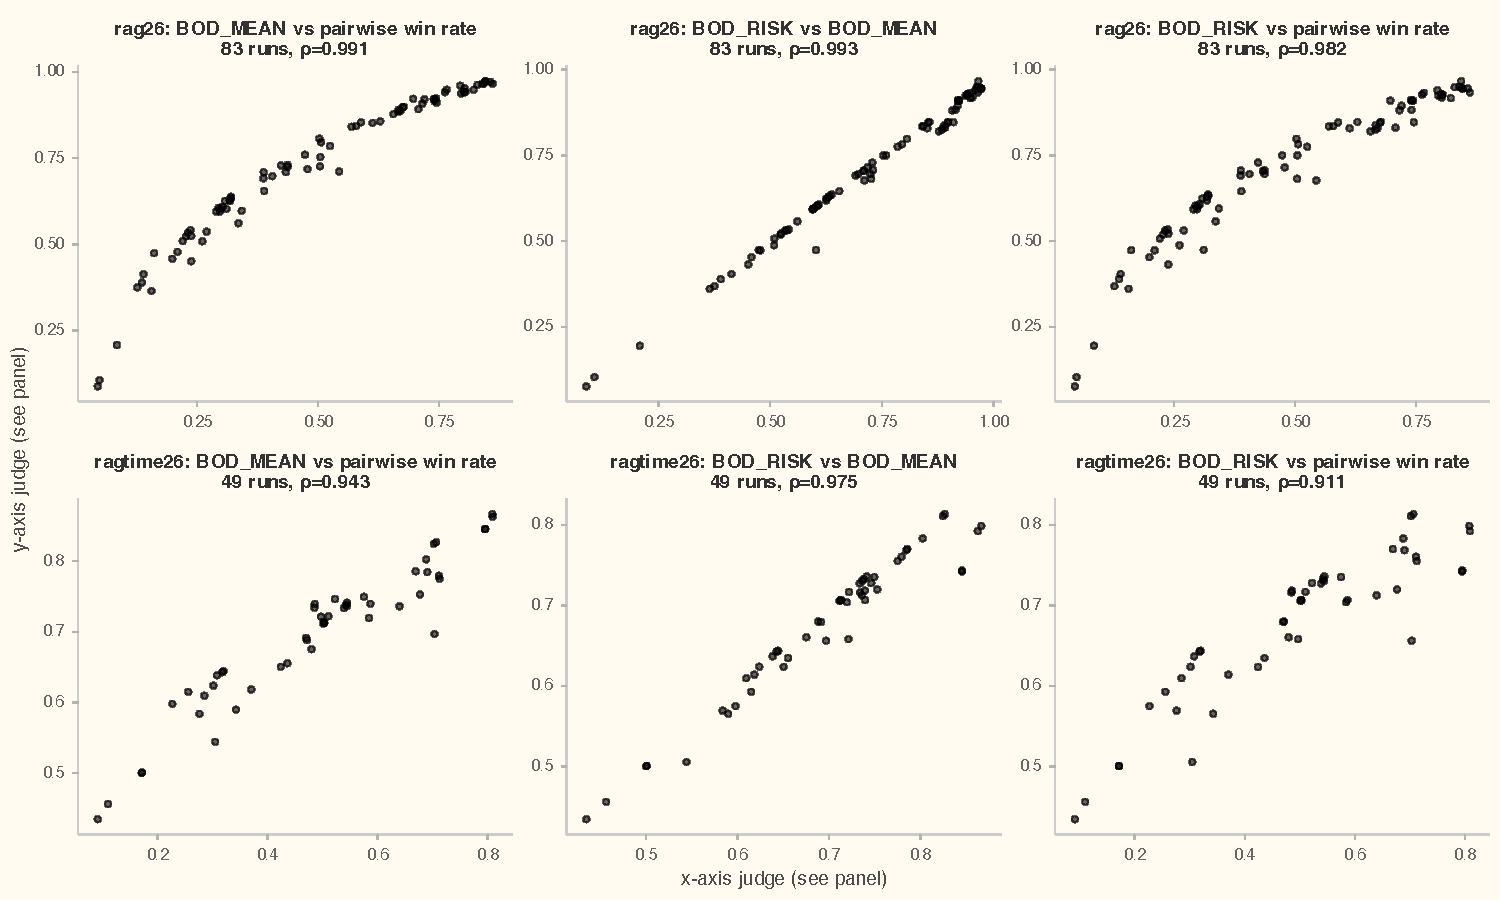
\includegraphics[width=1\linewidth,height=\textheight,keepaspectratio,alt={Submitted all-topic boards (``all'' rows): pairwise vs BOD ( 0.991 / 0.943), BOD vs BOD\_GROUNDED (0.993 / 0.975), pairwise vs BOD\_GROUNDED (0.982 / 0.911). Reporting only; not used for any decision.}]{figures_ggplot/f11_full_leaderboards.pdf}
\caption{Submitted all-topic boards (``all'' rows): pairwise vs BOD
(\ensuremath{\rho} 0.991 / 0.943), BOD vs BOD\_GROUNDED (0.993 / 0.975),
pairwise vs BOD\_GROUNDED (0.982 / 0.911). Reporting only; not used for
any decision.}\label{fig:f11}
\end{figure}

\begin{figure}
\centering
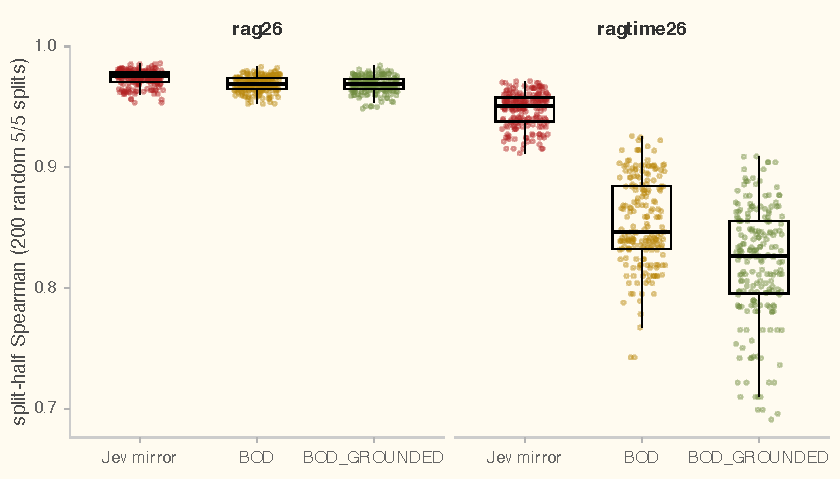
\includegraphics[width=0.6\linewidth,height=\textheight,keepaspectratio,alt={Split-half reliability on the window: Spearman between boards from two random 5-topic halves, 200 splits. Means: Jev mirror 0.974 / 0.948, BOD 0.969 / 0.854, BOD\_GROUNDED 0.968 / 0.820.}]{figures_ggplot/f12_split_half.pdf}
\caption{Split-half reliability on the window: Spearman between boards
from two random 5-topic halves, 200 splits. Means: Jev mirror 0.974 /
0.948, BOD 0.969 / 0.854, BOD\_GROUNDED 0.968 / 0.820.}\label{fig:f12}
\end{figure}

\subsection{8. Limitations}\label{limitations}

\begin{itemize}
\tightlist
\item
  \textbf{No ground truth.} Every result is about agreement, consistency
  or controlled sensitivity. Two judges that agree can share a bias, and
  LLM-judged leaderboards can be circular or gamed.
\item
  \textbf{The window is small and not random.} It is 10 topics per
  dataset, fixed by file order. Effects whose sign depends on the
  dataset (length, close-pair slot bias) may also vary across topics.
\item
  \textbf{Thin Gemini coverage.} The baseline covers 10 + 3 window
  topics, single orientation.
\item
  \textbf{Synthetic manipulations.}

  \begin{itemize}
  \tightlist
  \item
    The narrow requests were written by us.
  \item
    Padding splices may be easier to detect than real verbosity.
  \item
    pad\_relevant adds both information and text.
  \end{itemize}
\item
  \textbf{Model drift.} Results are reproducible from the cache. Fresh
  calls may differ: Jev 1.14 is now the latest version, and we pinned
  1.13.
\item
  \textbf{Rubrics.} BOD rubrics are generated from the topic only, so
  they can't credit useful content they didn't anticipate. Some needs
  are split into near-duplicate questions.
\item
  \textbf{Hallucination Risk is a lexical proxy.} It penalises correct
  paraphrase, depends on the pool of runs, and its definition was first
  explored on topics outside the window.
\end{itemize}

\begin{center}\rule{0.5\linewidth}{0.5pt}\end{center}

\subsection{9. Figures}\label{figures}

\begin{longtable}[]{@{}
  >{\raggedright\arraybackslash}p{(\linewidth - 6\tabcolsep) * \real{0.0744}}
  >{\raggedright\arraybackslash}p{(\linewidth - 6\tabcolsep) * \real{0.2479}}
  >{\raggedright\arraybackslash}p{(\linewidth - 6\tabcolsep) * \real{0.0826}}
  >{\raggedright\arraybackslash}p{(\linewidth - 6\tabcolsep) * \real{0.5950}}@{}}
\toprule\noalign{}
\begin{minipage}[b]{\linewidth}\raggedright
Figure
\end{minipage} & \begin{minipage}[b]{\linewidth}\raggedright
File
\end{minipage} & \begin{minipage}[b]{\linewidth}\raggedright
Section
\end{minipage} & \begin{minipage}[b]{\linewidth}\raggedright
Shows
\end{minipage} \\
\midrule\noalign{}
\endhead
\bottomrule\noalign{}
\endlastfoot
\ref{fig:f01} & f01\_probability\_distribution & §4.4 & Choice saturates
at 0/1; the mirror does not \\
\ref{fig:f03} & f03\_identical\_summaries & §4.4 & Identical summaries:
Choice \ensuremath{\approx} 0.79, mirror \ensuremath{\approx} 0.54 \\
\ref{fig:f02} & f02\_position\_bias & §4.4, §4.7 & P(slot A wins) by
closeness, Choice vs mirror \\
\ref{fig:f13} & f13\_determinism & §4.4 & Repeated identical requests \\
\ref{fig:f05} & f05\_prompt\_agreement & §4.5 & Ranking agreement
between four wordings \\
\ref{fig:f07} & f07\_broad\_narrow & §4.5 & Proportionate DiD per window
topic \\
\ref{fig:f04} & f04\_length & §4.6, §5.2 & P(longer wins) by length
ratio; per-topic \ensuremath{\rho}(score, words) for all judges \\
\ref{fig:f06} & f06\_padding & §4.6, §5.3 & Padding test: pairwise
judges and BOD \\
\ref{fig:f08} & f08\_judge\_agreement & §4.2, §5.2 & Window boards: Jev
vs Gemini, BOD vs Jev \\
\ref{fig:f09} & f09\_bod\_grades & §5.2 & BOD grade distributions \\
\ref{fig:f10a} & f10a\_hallucination\_risk & §6.2 & Risk
distributions \\
\ref{fig:f10b} & f10b\_grounded\_vs\_mean & §6.2 & BOD\_GROUNDED vs
BOD\_MEAN \\
\ref{fig:f11} & f11\_full\_leaderboards & §7 & Submitted all-topic
boards against each other \\
\ref{fig:f12} & f12\_split\_half & §4.8, §7 & Split-half reliability per
judge \\
\end{longtable}

Draft captions with exact values are in
\passthrough{\lstinline!papers/figures/CAPTIONS.md!}.

\begin{center}\rule{0.5\linewidth}{0.5pt}\end{center}

\subsection{Appendix A. Prompts and questions
(verbatim)}\label{appendix-a.-prompts-and-questions-verbatim}

\subsubsection{A.1 Submitted pairwise question (Noul, asked as a
mirrored
pair)}\label{a.1-submitted-pairwise-question-noul-asked-as-a-mirrored-pair}

\begin{quote}
You are a subject matter expert. Two RAG summaries (summary\_a and
summary\_b) were generated for the query. Does summary\_a
{[}summary\_b{]} satisfy the information need of the query better than
summary\_b {[}summary\_a{]} does, considering relevance, completeness,
depth proportionate to what the query asks for (thorough when the query
is broad or multi-part, brief and direct when it is narrow), and how
well its claims are grounded?
\end{quote}

\begin{itemize}
\tightlist
\item
  \textbf{true:} summary\_a {[}summary\_b{]} satisfies the information
  need of the query better than summary\_b {[}summary\_a{]}, at a depth
  proportionate to what the query asks for.
\item
  \textbf{false:} summary\_a {[}summary\_b{]} does not satisfy the
  information need of the query better than summary\_b {[}summary\_a{]},
  at a depth proportionate to what the query asks for.
\end{itemize}

Request shape:
\passthrough{\lstinline!\{"model": "typesafe/jev-1.13", "state": \{"query", ["problem\_statement"], ["background"], "summary\_a", "summary\_b"\}, "questions": \{...\}\}!}.

\subsubsection{A.2 BOD rubric prompt (Gemini 2.5 Flash Lite, temperature
0)}\label{a.2-bod-rubric-prompt-gemini-2.5-flash-lite-temperature-0}

\begin{lstlisting}
You are designing a grading rubric for answers to a user's information need.

<information_need>
<%=topic_query%>
</information_need>

Write the questions a careful expert would use to grade how well an answer meets this information need. Each question checks one distinct part of what the user needs to know or do.

Rules:

- Write between <%=min_questions%> and <%=max_questions%> questions. Use as many as the need has genuinely distinct parts: a narrow, single-fact need gets few questions; a broad, multi-part need gets more. Do not pad the list to reach a number.
- Each question must be gradable on a scale from "not addressed" to "fully answered with specific detail", so phrase it as "Does the answer ...?" about content, e.g. "Does the answer explain why ...?" or "Does the answer give ...?".
- Every question must check substantive content: a fact, explanation, step, or piece of advice the user asked for or clearly needs to act on what they asked.
- Use any background or situation described only to decide WHAT content the user needs (for example, a safety concern makes safety advice necessary). Do not write questions that merely check whether the answer acknowledges, mentions, or relates to the user's interests, hobbies, or feelings.
- No two questions may check the same thing. Do not ask about tone, reading level, style, length, formatting, or citations.
- Do not mention any particular source, product, or answer.

Return ONLY a JSON array of strings, one per question, with no other text.
\end{lstlisting}

\subsubsection{A.3 BOD grade question (Jev Choice, one per rubric
question)}\label{a.3-bod-grade-question-jev-choice-one-per-rubric-question}

\begin{lstlisting}
{
  "type": "choice",
  "instructions": "Grade the answer on this question: <rubric question>",
  "criteria": {
    "0": "The answer does not address this question at all.",
    "1": "The answer mentions this topic but gives no real substance or explanation.",
    "2": "The answer partially answers this question; important parts are missing or vague.",
    "3": "The answer fully answers this question with specific, accurate detail."
  }
}
\end{lstlisting}

Padding question (Noul): ``Does the answer contain substantial content
that is off-topic, repeated, or generic filler that does not help with
the user's question?''

\subsubsection{A.4 Gemini baseline
prompt}\label{a.4-gemini-baseline-prompt}

Verbatim in notes §18.1: the query, both summaries, and an instruction
to answer with exactly one character, \passthrough{\lstinline!A!} or
\passthrough{\lstinline!B!}.

\begin{center}\rule{0.5\linewidth}{0.5pt}\end{center}

\subsection{References to cite}\label{references-to-cite}

Numbers in brackets are the reference numbers in notes §19, which has
the full entries and URLs. \passthrough{\lstinline!papers/prompt.md!}
uses the same list.

\begin{itemize}
\tightlist
\item
  \textbf{Tracks and infrastructure:} TREC AutoJudge {[}1{]}, HowTo and
  data policy {[}2{]}, TREC RAG site, Ragnarök baselines and 2025
  overview {[}4, 5, 6{]}, RAGTIME site and 2025 overview {[}7, 8{]},
  report evaluation {[}9{]}, TIRA {[}10, 11{]}, ir\_measures {[}12{]},
  trec\_eval {[}13{]}.
\item
  \textbf{RAG evaluation and nuggets:} AutoNuggetizer {[}14{]}, Great
  Nugget Recall {[}15{]}, support evaluation {[}16{]}, TREC QA nuggets
  {[}17, 18{]}, automatic nugget matching {[}19, 20{]}, Pyramid method
  {[}21{]}.
\item
  \textbf{LLMs as assessors:} Thomas et al.~{[}22{]}, UMBRELA {[}23{]},
  LLMJudge {[}24{]}, LLM4Eval {[}25{]}, Faggioli et al.~{[}26{]}, Clarke
  and Dietz {[}27{]}, Alaofi et al.~{[}28{]}, Arabzadeh and Clarke
  {[}29{]}, Pencils Down {[}30{]}.
\item
  \textbf{Pairwise and preference judging:} Carterette et al.~{[}31{]},
  Clarke et al.~{[}32{]}, MT-Bench {[}33{]}, PRP {[}34{]},
  LLM-as-a-judge survey {[}35{]}, Bradley--Terry {[}36{]}, Chatbot Arena
  {[}37{]}.
\item
  \textbf{Position and length bias:} {[}33{]}, Wang et al.~{[}38{]}, Shi
  et al.~{[}39{]}, Saito et al.~{[}40{]}, length-controlled AlpacaEval
  {[}41{]}.
\item
  \textbf{Jev:} OpenRouter documentation {[}3{]}, Decisions API
  {[}42{]}, Jev as a reranker {[}43{]}, Bag of Decisions Reranker
  {[}44{]}.
\item
  \textbf{Statistics and protocol:} pre-registration {[}45{]}, Sakai's
  bootstrap {[}46{]}, Kendall {[}47{]}, Voorhees {[}48{]}.
\item
  \textbf{Rubric judges:} Pencils Down {[}30{]}, LLM-Rubric {[}49{]},
  Prometheus {[}50{]}, FLASK {[}51{]}, G-Eval {[}52{]}.
\item
  \textbf{Hallucination and grounding:} concept F1 {[}53{]}, RAGAS
  {[}54{]}, spaCy and \passthrough{\lstinline!en\_core\_web\_lg!} {[}55,
  56{]}, SelfCheckGPT {[}57{]}, FActScore {[}58{]}, AIS {[}59{]}, ALCE
  {[}60{]}, ARES {[}61{]}, verifiability {[}62{]}, surveys {[}63, 64{]},
  ROUGE {[}65{]}.
\end{itemize}

\end{document}
